\documentclass[12pt]{book}
\usepackage[width=4.375in, height=7.0in, top=1.0in, papersize={5.5in,8.5in}]{geometry}
%\usepackage[pdftex]{graphicx}
\usepackage{amsmath}
\usepackage{amssymb}
\usepackage{tipa}
%for using the euro sign
\usepackage{eurosym}
\usepackage{graphicx}
%\usepackage{txfonts}
\usepackage{textcomp}
%\usepackage{amsthm}
\usepackage{array}
%\usepackage{xy}
\usepackage{fancyhdr}

\usepackage{hyperref}

%Ommit some vbox and hbox errors (under 10000)
\vbadness=10000
\hbadness=10000

%The below is used for codes
\usepackage{color}

\definecolor{dkgreen}{rgb}{0,0.6,0}
\definecolor{gray}{rgb}{0.75,0.75,0.75}
\definecolor{mauve}{rgb}{0.58,0,0.82}
\usepackage{listings}
\lstset{
  backgroundcolor=\color{gray},  % choose the background color; you must add \usepackage{color} or \usepackage{xcolor}
  basicstyle=\footnotesize,       % the size of the fonts that are used for the code
  breakatwhitespace=false,        % sets if automatic breaks should only happen at whitespace
  breaklines=true,                % sets automatic line breaking
  captionpos=b,                   % sets the caption-position to bottom
  commentstyle=\color{dkgreen},   % comment style
  deletekeywords={...},           % if you want to delete keywords from the given language
  escapeinside={@}{@)},         % if you want to add LaTeX within your code
  %extendedchar=true,              % lets you use non-ASCII characters; for 8-bits encodings only, does not work with UTF-8
  frame=single,                   % adds a frame around the code
  keywordstyle=\color{mauve},      % keyword style
  language=C,                % the language of the code
  morekeywords={*,...},           % if you want to add more keywords to the set
  numbers=left,                   % where to put the line-numbers; possible values are (none, left, right)
  numbersep=5pt,                  % how far the line-numbers are from the code
  numberstyle=\tiny\color{dkgreen},  % the style that is used for the line-numbers
  rulecolor=\color{black},        % if not set, the frame-color may be changed on line-breaks within not-black text (e.g. comments (green here))
  showspaces=false,               % show spaces everywhere adding particular underscores; it overrides 'showstringspaces'
  showstringspaces=false,         % underline spaces within strings only
  showtabs=false,                 % show tabs within strings adding particular underscores
  stepnumber=1,                   % the step between two line-numbers. If it's 1, each line will be numbered
  stringstyle=\color{mauve},      % string literal style
  tabsize=4,                      % sets default tabsize to 2 spaces
  title=\lstname,                  % show the filename of files included with \lstinputlisting; also try caption instead of title
}
%until here

\newcommand{\tab}{\hspace*{2em}}


\pagestyle{fancy}
\renewcommand{\chaptermark}[1]{\markboth{#1}{}}
\renewcommand{\sectionmark}[1]{\markright{\thesection\ #1}}
\fancyhf{}
\fancyhead[LE,RO]{\bfseries\thepage}
\fancyhead[LO]{\bfseries\rightmark}
\fancyhead[RE]{\bfseries\leftmark}
\renewcommand{\headrulewidth}{0.5pt}
\renewcommand{\footrulewidth}{0pt}
\addtolength{\headheight}{0.5pt}
\setlength{\footskip}{0in}
\renewcommand{\footruleskip}{0pt}
\fancypagestyle{plain}{%
\fancyhead{}
\renewcommand{\headrulewidth}{0pt}
}
%
%\parindent 0in
\parskip 0.05in
%
\begin{document}
\frontmatter
\pagestyle{empty}
%\pagenumbering{}
% Set book title
\title{\textbf{A course on Wireless Sensor Networks (WSNs)}}
% Include Author name and Copyright holder name
\author{Luis Sanabria, Jaume Barcelo}
% 1st page for the Title
%-------------------------------------------------------------------------------
\maketitle
%
\tableofcontents
%
\mainmatter
%
\chapter*{Acknowledgements}

We would like to thank all the people involved in the development of both the first, and this second edition of the course guide. Further, we are also immensely greatful for all the collaboration and feedback we have got regarding the \emph{\color{blue}{\href{http://handsonwsn.org/}{Hands-on WSN community}}}.

Thanks Laia Alb\'{o}, Alejandro Andreu and Javier L\'{o}pez for your dedication and infinite patience.

\chapter{About the course}

\section{Course Data}

Code: 21754

Course name: ``Xarxes de Sensors Sense Fils''

Teacher: Luis Sanabria and Jaume Barcelo

Credits: 4

Year: 3rd or 4th year (optional)

Trimester: Spring

\section{Introduction}
The reduction in price and size of computing and wireless communication platforms over the last years opens a new possibility for gathering and processing information: Wireless Sensor Networks.
A wireless sensor node is an electronic device of small dimensions that gathers measures from the environment and transmit the data wirelessly.
In wireless sensor nodes, communication is often established with other wireless sensor nodes to exchange or pass information.
It is common to have this data directed to an special device that gathers all the data and is called the network sink.
As wireless sensor nodes are often battery-powered, energy saving is a relevant issue in these networks.

What follows is an extract of the first pages of \cite{sanabria2012lpw}.

\begin{quotation}
Wireless Sensor Networks (WSNs) are a result of significant breakthroughs on wireless transceiver technology, the need of event sensing and monitoring. One might think of a WSN as the skin of our bodies; apart from its importance on many other subjects, our skin senses events nearby it, like touch, temperature changes, pressure and so forth. These events are generated by an external entity, the nerves or sensors of our skin are capable to react to such events and transmit this information to the brain. \\

There are enormous differences among characteristics of WSN and the skin, but the example given above will work as head start to understanding the technology. For instance, our skin sends the sensed event information towards the brain through the nerves, we could safely relate this medium to a wired network infrastructure. While in WSN, as its name suggests sends the sensed data towards a central node (Sink) via a wireless medium. Because of the limited radio range of each node, the route to the Sink is generally composed of jumps through different nodes (which is called a multi-hop route).\\

The majority of wireless nodes in a WSN are very constrained devices due to the restrictions in costs and sometimes harsh environments where these networks are deployed. These constraints go from cost, processing power, memory, storage, radio range, spectrum and, more importantly, battery life. One of the most popular low-end nodes model, the TelosB, is equipped with $16$ MHz CPU, very small flash memory ($48$ KB avg.), about $10$ KB of RAM and works on the very crowded $2.4$ GHz spectrum at rates around $250$ Kbps. These limitations force WSN engineers to design applications capable of working with low processor-intensive tasks and powered with limited battery (usually two AA batteries).\\

Many WSN applications process the sensed event before sending the data, this processing tries to reduce the information to send. As mentioned in \cite{akyildiz2010wireless}, it is less energy consuming to process one bit of information than sending it. WSN protocols and applications are tailored to power conservation rather than throughput, mainly due to cost, dimension, processing and power constraints.\\

WSNs may contain different kind of sensors that help monitor metrics related to: temperature, humidity, pressure, speed, direction, movement, light, soil makeup, noise levels, presence or absence of certain kinds of objects, mechanical stress and vibration. Also further information like node location can be derived from a Global Positioning System (GPS) device embedded at each node.\\

Because of the variety of measures than can be monitored with these small and (generally) cheap devices, a wide range of applications have been developed; the authors of \cite{akyildiz2010wireless} divide them in: military, environmental, health, home and industry applications.\\

\begin{itemize}
    \item \emph{Military Applications:} one of the first applications of WSNs. The main advantages in this area are the fact that the deployment of low cost sensors (that are subject to destruction in a battlefield) proposes a cheaper approach to sensing different types of metrics, which in turn brings new challenges to WSN applications (increased power and processing constraints). Some of the applications are related to: monitoring the movement of troops, equipment and ammunition, battlefield surveillance, terrain reconnaissance, damage assessments, snipper detection \cite{ledeczi2005countersniper}, \cite{mazurek2005boomerang} and threat detection, as in the case of biological, radiological or chemical attacks.\\
    \item \emph{Environmental Applications:} most of these applications are related to animal tracking, weather conditions and threat contention \cite{polastre2004analysis}, \cite{szewczyk2004habitat}.\\
    \item \emph{Health Applications:} a great deal of these applications are dedicated to monitor patients inside hospitals and provide them with better care. This is achieved by tracking the patientÕs vitals or other information of interest and making it available to doctors at any time from anywhere securely through the Internet. \\
    \item \emph{Home Applications:} technology is making its way inside our homes from various fronts, and WSN are no exception. Sensor nodes inside domestic devices will result in an increased interaction among them and allow access via the Internet. Theses applications are of great importance in fields like domotics towards a smart home/work environment. Home surveillance and multimedia WSNs for home environments are also a growing field of research.\\
    \item \emph{Industrial Applications:} historically the monitoring of material fatigue was made by experts introducing the observed situation inside PDA devices to be collected on a central site for processing. Further sensing techniques were developed on the form of wired sensors; nevertheless its implementation was slow and expensive due the necessary wiring. WSNs bring the best of both methods by sensing the events without the need of expert personnel and the cost of wiring. \\
    \item Other implementations as mentioned in \cite{akyildiz2010wireless} are: inventory management, product quality monitoring, smart offices/houses; guidance in automatic manufacturing environments, interactive museums, factory process control and automation, machine diagnosis, transportation, vehicle tracking and detection, spectrum sensing for cognitive radio networks, underground and underwater monitoring. \\
\end{itemize}

\end{quotation}

\section{Syllabus}
\begin{itemize}
  \item Lectures
  \begin{enumerate}
    \item Introduction to WSNs.
    \item Arduino Platform.
    \item XBee and XBee explorer. AT commands.
    \item XBee API mode.
    \item A sensor network with Arduino.
    \item A sensor network without Arduino.
    \item Publishing sensed data
    \item Invited talk
    \item Quiz
  \end{enumerate}
  \item Labs and seminars
  \begin{enumerate}
    \item Blinking LED (Dimming optional)
    \item Blinking LED with push-button (dimming optional)
    \item XBee chat
    \item Wireless doorbell
    \item Sunset sensor
    \item Sensor network with Arduino
    \item Sensor network with XBee in API mode
    \item Sleeping and actuating
    \item Uploading sensed data to the Internet
  \end{enumerate}
\end{itemize}

\section{Bibliography}

Most of the lab assignments follow the book that you can find at the university library:

Robert Faludi ``Building Wireless Sensor Networks'' (\cite{faludi2010bws}).

The following list of ``common mistakes'' can be very useful when debugging your projects:

\url{http://www.faludi.com/projects/common-xbee-mistakes/}

Check also:

Massimo Banzi ``Getting Started with Arduino''.

\section{Evaluation Criteria}

The grading is distributed as follows:
\begin{itemize}
\item Quiz, 10\%
\item Each lab assignment, 10\%
\end{itemize}

It is necessary to obtain a decent mark in all the different evaluation aspects.
To pass the course, 50 out of the total 100 points need to be obtained.

\section{Team work}

You will work in teams of three people.
Try to make the groups as heterogeneous as possible: people that are experienced with Arduino and people that are not, people from different majors, people with strong programming skills and people good at electronics, etc.

Each group delivers a single report per session and the teachers may ask questions to individual members of the team.

\section{Use your imagination}
The lab assignments are somewhat easy.
The goal is that you complement what you do in the lab with other ideas of your own.
You are encouraged to explore WSNs beyond the basics introduced in the assignments and document your findings in the reports.
Doing something on your own beyond the assignment takes a lot of effort and is time-consuming.
Nevertheless, as engineers, we should be able to come up with new ideas and solutions on our own.

\section{Non-stop Arduino}
In our school there are two additional courses that make use Arduino: ``Sensors and data acquisition'' and ``Interactive Systems''.

\section{Survival guide}

\subsection{Questions and doubts}
We like to receive questions and comments.
Normally, the best moment to express a doubt is during the class, as it is likely that many people in the class share the same doubt.
If you feel that you have a question that needs to be discussed privately, we can discuss it right after the class.

\subsection{Continuous feedback}
At the end of the lecture, we will ask you to anonymously provide some feedback on the course \emph{\color{blue}{\href{http://bit.ly/10tXjX4}{using a form like this one}}}.
In particular, I always want to know:
\begin{itemize}
\item What is the most interesting thing we have seen in class.
\item What is the most confusing thing in the class.
\item Any other comment you may want to add.

In labs, I will ask each group to hand in a short (few paragraphs) description of the work carried out in class, and the members of the group that have attended the class.
Note that this is different from the deliverables, which are the ones that are actually graded.
\end{itemize}

\subsection{How to make you teachers happy}

Avoid speaking while we are talking.

\chapter{Introduction to Arduino}

\section{Open Hardware}
\emph{"There's a fine line between open source and stupidity"}, says Massimo Banzi to a reporter from Wired Magazine while having dinner at a restaurant in Milan. 

Banzi is the man behind Arduino, an open hardware platform. The open about it relates to the fact that the device's manufacturing schematics, programming language and software development environment are free and open source. This basically means that everyone interested on building hardware-coupled solutions may take an Arduino board's schematics, modify it at will, send the new design to a China manufacturer and get the final product back home for around \EUR{10}~\cite{wiredOpenHardware}.

Open hardware is supported by a variety of available licenses (like open software with LGPL, GPL, Copyleft, and others) that ensure that the protected platform can be copied, enhanced and even sold, but always recognizing the original authors. It also ensures that the resulting products are open as the original.

\section{The Arduino Platform}
Arduino was developed to teach Interaction Design~\cite{banzi2008getting}, that meant that it required the ability to sense the surroundings and do something about it.

The platform is equipped with simple digital and analog input/output interfaces, that can be programmed to sense or react to some events. Figure~\ref{fig:ArduinoBoard} shows the Arduino Duemilanove board.

\begin{figure}[htbp]
  \centering
  \includegraphics[width=0.7\linewidth]{figures/duemilanove.eps}
  \caption{Arduino Duemilanove board
  \label{fig:ArduinoBoard}}
\end{figure}

There are numerous sensors and actuators that work with Arduino. In relation to sensors: temperature, air pollution, light, GPS modules and sound are among the popular; as LEDs, speakers and digital/analog outputs are common actuators. Also, interfaces like buttons can be programmed and used as a human interactive input.

The design and electrical components of the Arduino board are available for anyone~\cite{Arduino}. Figure~\ref{fig:Arduino_schematics} shows the connections layout of the Duemilanove model (see Figure~\ref{fig:ArduinoBoard}).

\begin{figure}[htbp]
  \centering
  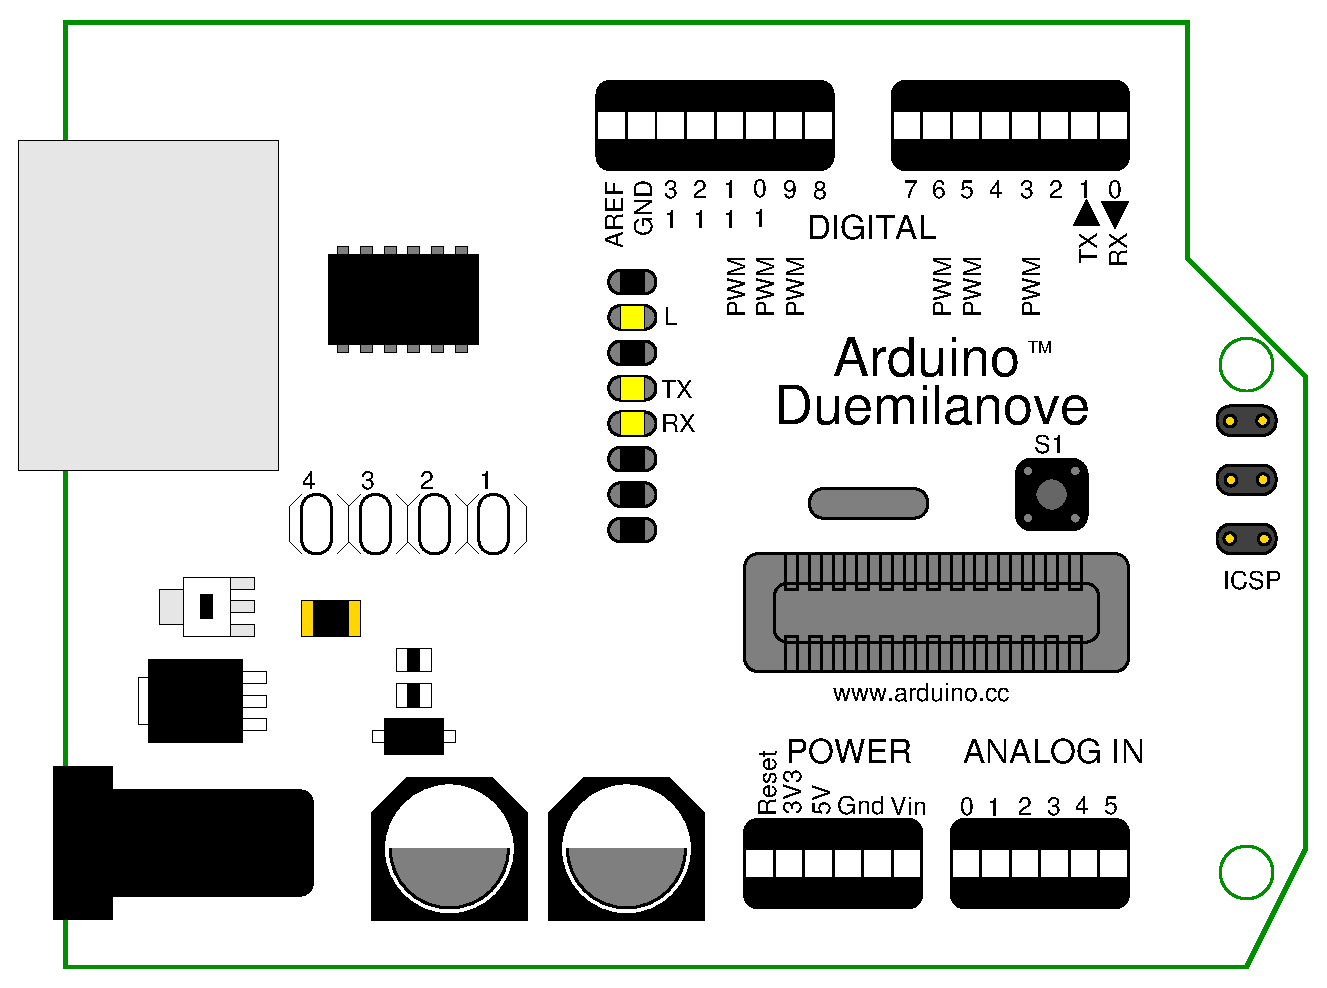
\includegraphics[width=0.7\linewidth]{figures/duemilanove_layout.eps}
  \caption{Arduino Duemilanove board: layout
  \label{fig:Arduino_schematics}}
\end{figure}

% \subsection{Developing for Arduino}

% \subsection{Example of a simple Arduino application}
	\chapter{Practice: Installing the Arduino IDE}\label{pract:settingTheIDE}
\section*{Suggested read: Chaper~ \ref{introToArduino}}

In the following practice, you will spend some time getting to know the Arduino platform, its connections and how to interact with it through a PC.

\section{Reviewing the hardware}\label{pract:settingTheIDE:hardware}
As you were able to see in Figure~\ref{fig:Arduino_schematics}, the Arduino board contains a whole computer on a small chip, although it is at least a thousand times less powerful.

Taking a closer look at Figure~\ref{fig:Arduino_schematics}, you will be able to see \emph{14 Digital IO pins (pins 0-13), 6 Analogue IN pins (0-5) and 6 Analogue OUT pins (pins 3, 5, 6, 9, 10, and 11)}.

The \emph{Digital IO} pins, as the name suggests can be set to input or output. Their function is specified by the sketch you create in the IDE (more on IDE in Section~\ref{pract:settingTheIDE:IDE}). The \emph{Analogue IN} ports take analogue values (i.e., voltage readings from a sensor) and convert them into a number between 0 and 1023. As for the \emph{Analogue OUT} ports, are actually digital pins that can be reprogrammed for analogue output using the sketch you can create in the IDE.

\section{The Arduino IDE}\label{pract:settingTheIDE:IDE}
The Arduino Integrated Development Environment (IDE) is the responsible for making your code work in the Arduino board. Without entering in much unnecessary detail, what the IDE does is to translate your code into C language and compile it using \texttt{avr-gcc}, which makes it understandable to the micro-controller. This last step hides away as much as possible the complexities of programming micro-controllers, so you can spend more time thinking on your actual code.

You can download the Arduino IDE~\emph{\color{blue}{\href{http://www.arduino.cc/en/Main/Software}{from here}}}. If you are using \emph{Linux} or \emph{Windows} operating systems, just double click the downloaded file. This will open a folder named \emph{arduino-[version]}, such as \emph{arduino-1.0}. Place the folder wherever you want in your system. For Ubuntu users, a good alternative is to use the \emph{Ubuntu Software Center} when available. On the Mac, just double click the downloaded file, this will open a disk image containing the Arduino application. Drag a drop the application icon to your Applications folder.

Do not open your installed application yet. First you must teach your computer to detect the Arduino hardware through the USB ports.

\subsection{Configuring the USB ports for detecting the Arduino}
In Linux and OS X, the USB controllers are the same used by the operating system.

\emph{\bf{On the Mac}}, plug the Arduino into an USB port.

The PWR light on the board should come on. Also, the LED labelled "L" should start blinking.

Then, a pop-up window telling you that a new network interface was found should appear. Proceed clicking "Network Preferences...", and then "Apply". Although it may appear with a status of "Not Configured", the Arduino is ready for work.

\emph{\bf{Windows}} machines, plug your Arduino and the ``Found new Hardware Wizard'' will appear. After the wizard tries to find the driver on the Internet, you will be able to select "Install from a list or specific location" button. Choose it and click next. You will be able to find the drivers under the "Drivers" folder of the Arduino Software download.

Once the drivers are installed, you can launch the IDE and start using Arduino.

\subsection{Identifying the port connected to the Arduino}
In the case of the \emph{\bf{Mac}}, once in the Arduino IDE, select "Serial Port" from the "Tools" menu. Select \texttt{/dev/cu/.usbmodem}; this is the name that your computer uses to refer to the Arduino board.

For \emph{\bf{Windows}}, under the operating system "Start" menu open the "Device Manager" by right-clicking on "Computer" (Vista) or "My Computer" (XP), then choose properties. On XP, click "Hardware" and choose Device Manager. On Vista, click "Device Manager".

Look for the Arduino device in the list under "Ports (COM \& LPT)". Your device name will be followed by a port number, usually "COM\#", where \# refers to a number.

Once you have identified the COM port number for the Arduino connection, you can select that port from the Tools~$>$~Serial Port menu in the Arduino IDE.

Now the Arduino IDE can talk with the Arduino board and program it.

\subsection{What's the deal with Linux users?}
As mentioned before, IDE uses the same USB controllers than Linux. So, in order to effectively detect your Arduino in Linux, simply connect it to your PC, open a Terminal a type \texttt{ls /dev/tty*}. This will display all available ports. Your Arduino serial port will probably be something like \texttt{/dev/ttyUSB0} or \texttt{/dev/ttyACM0}, but you can be sure by typing \texttt{dmesg} in the Terminal and looking at the line that details the last connected USB device to a determined \texttt{/dev/tty*} port.
	\chapter{Practice: Blinking LED}\label{pract:blinkingLED}
\section*{Suggested read: Chapers~\ref{introToArduino}~and~\ref{pract:settingTheIDE}}

In the following practice you will write your first Arduino application. Although simple, mastering it will provide you with clear understanding of the IDE and the components that conform the Arduino platform.

It consist of a simple code that will turn on/off LED(s) plugged to the digital IO ports of the Arduino.

\section{Preparing your development environment}
For Practice~\ref{pract:blinkingLED}, you will need:
\begin{itemize}
 \item as many LEDs as you want, but always less than the number of digital IO ports.
 \item a USB cable to connect your Arduino board to the PC.
 \item the Arduino IDE, up and running.
\end{itemize}

Turn your Arduino on by plugging it to the PC. Make sure you have selected the appropriate COM port, as it is explained in Practice~\ref{pract:settingTheIDE} according with your operating system.

\section{The code} 
Once inside, enter the following code:

\begin{lstlisting} [caption = {Blinking LED example code}, language = C, label = {code:blinkingLED}, numbers = left, escapeinside={@}{@}]
const int LED = 13; @\label{BL:LED}@

void setup() @\label{BL:SETUP}@
{
	pinMode(LED,OUTPUT); @\label{BL:pinMODE}@
}

void loop() @\label{BL:LOOP}@
{
	digitalWrite(LED, HIGH); @\label{BL:HIGH}@
	delay(1000); @\label{BL:DELAY}@
	digitalWrite(LED, LOW); @\label{BL:LOW}@
	delay(1000); @\label{BL:DELAY2}@
}
\end{lstlisting}

As you might be able to see, the code is completely readable. Let's review it line by line.

\begin{itemize}
	\item Line~\ref{BL:LED}: \texttt{const int LED = 13}, assigns the value $13$ to a \texttt{\color{red}{int}}erger variable, named LED. In this case, this number corresponds to the digital IO port \#13.
	\item Line~\ref{BL:SETUP}: \texttt{void setup()} is the name of the next block of code. It is very similar to functions in languages like C/C++ and it is generally used to assign variables to ports, as well as their role.
	\item Line~\ref{BL:pinMODE}: \texttt{pinMode(LED,OUTPUT)} tells the Arduino how to set the pins. In this case, pin LED ($\#13$) is set up as an OUTPUT. \texttt{pinMode} is a function, and the words or numbers inside the parenthesis are its arguments.
	\item Line~\ref{BL:LOOP}: \texttt{void loop()}: is where you define the behaviour of your device. The statements contained in \texttt{loop()} are repeated over and over again until the device is turned off.
	\item Line~\ref{BL:HIGH}: \texttt{digitalWrite(LED, HIGH)} works as a power socket for pins. In this case, the command is indicating to turn pin \texttt{LED} into \texttt{HIGH}, which instructs Arduino to turn the output pin to $5$V. If you have connected a LED in this pin, the result is that it will turn on (hopefully). Turning on and off the pin allow us to see what the software is making the hardware do; the LED is an actuator.
	\item Line~\ref{BL:DELAY}: \texttt{delay(1000)} tells the processor to wait for $1000$ \emph{milliseconds} before proceeding to the next code line.
	\item Line~\ref{BL:LOW}: \texttt{digitalWrite(LED, LOW)} as with Line~\ref{BL:HIGH}, this function turns pin \texttt{LED} to $0$V, causing the connected LED to turn off. You can do a mental map in which $HIGH \rightarrow ON,\ LOW \rightarrow OFF$.
	\item Line~\ref{BL:DELAY2}: because the last instruction was to set the LED off, this will keep it that way for an additional $1000$ \emph{millisecods}.
\end{itemize}

To see your work, just insert the longer leg of the LED into the digital IO port you assigned to variable \texttt{LED} on your code (digital pin $13$), and the shorter leg to ground (GND). Figure~\ref{fig:blinkingLEDLayout} shows the desired layout.

\begin{figure}[htbp]
  \centering
  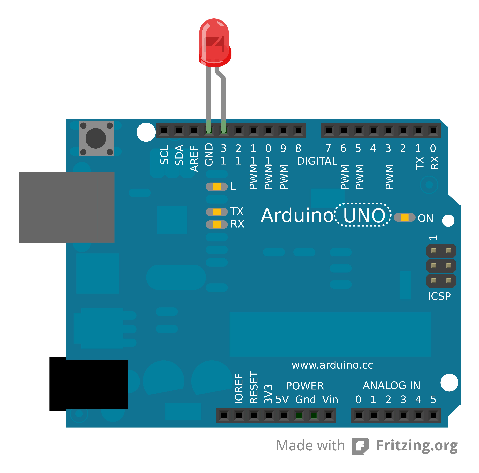
\includegraphics[width=0.7\linewidth]{figures/blinkingLED-NEW.eps}
  \caption{Blinking LED layout
  \label{fig:blinkingLEDLayout}}
\end{figure}

	\section{Practice: Blinking LED Advanced}\label{pract:blinkingLEDAdvanced}

It will be very boring to just have a blinking LED. That is because in this practice we will be incorporating some hardware and software tweaks that will allow us to have a little more control over the LED. Or let's say, we will make a basic lamp.

What we want to prototype is a LED that turns on or off whenever we press a bottom. Before we dwell into detail, let's review what we will need:

\begin{itemize}
	\item A breadboard (we will be using Figure~\ref{fig:breadboard} as a guide).
	\item Wire to tie together the different parts of your circuit.
	\item One $10$K Ohm resistor.
	\item One pushbutton switch.	
\end{itemize}

\begin{figure}[htbp]
  \centering
  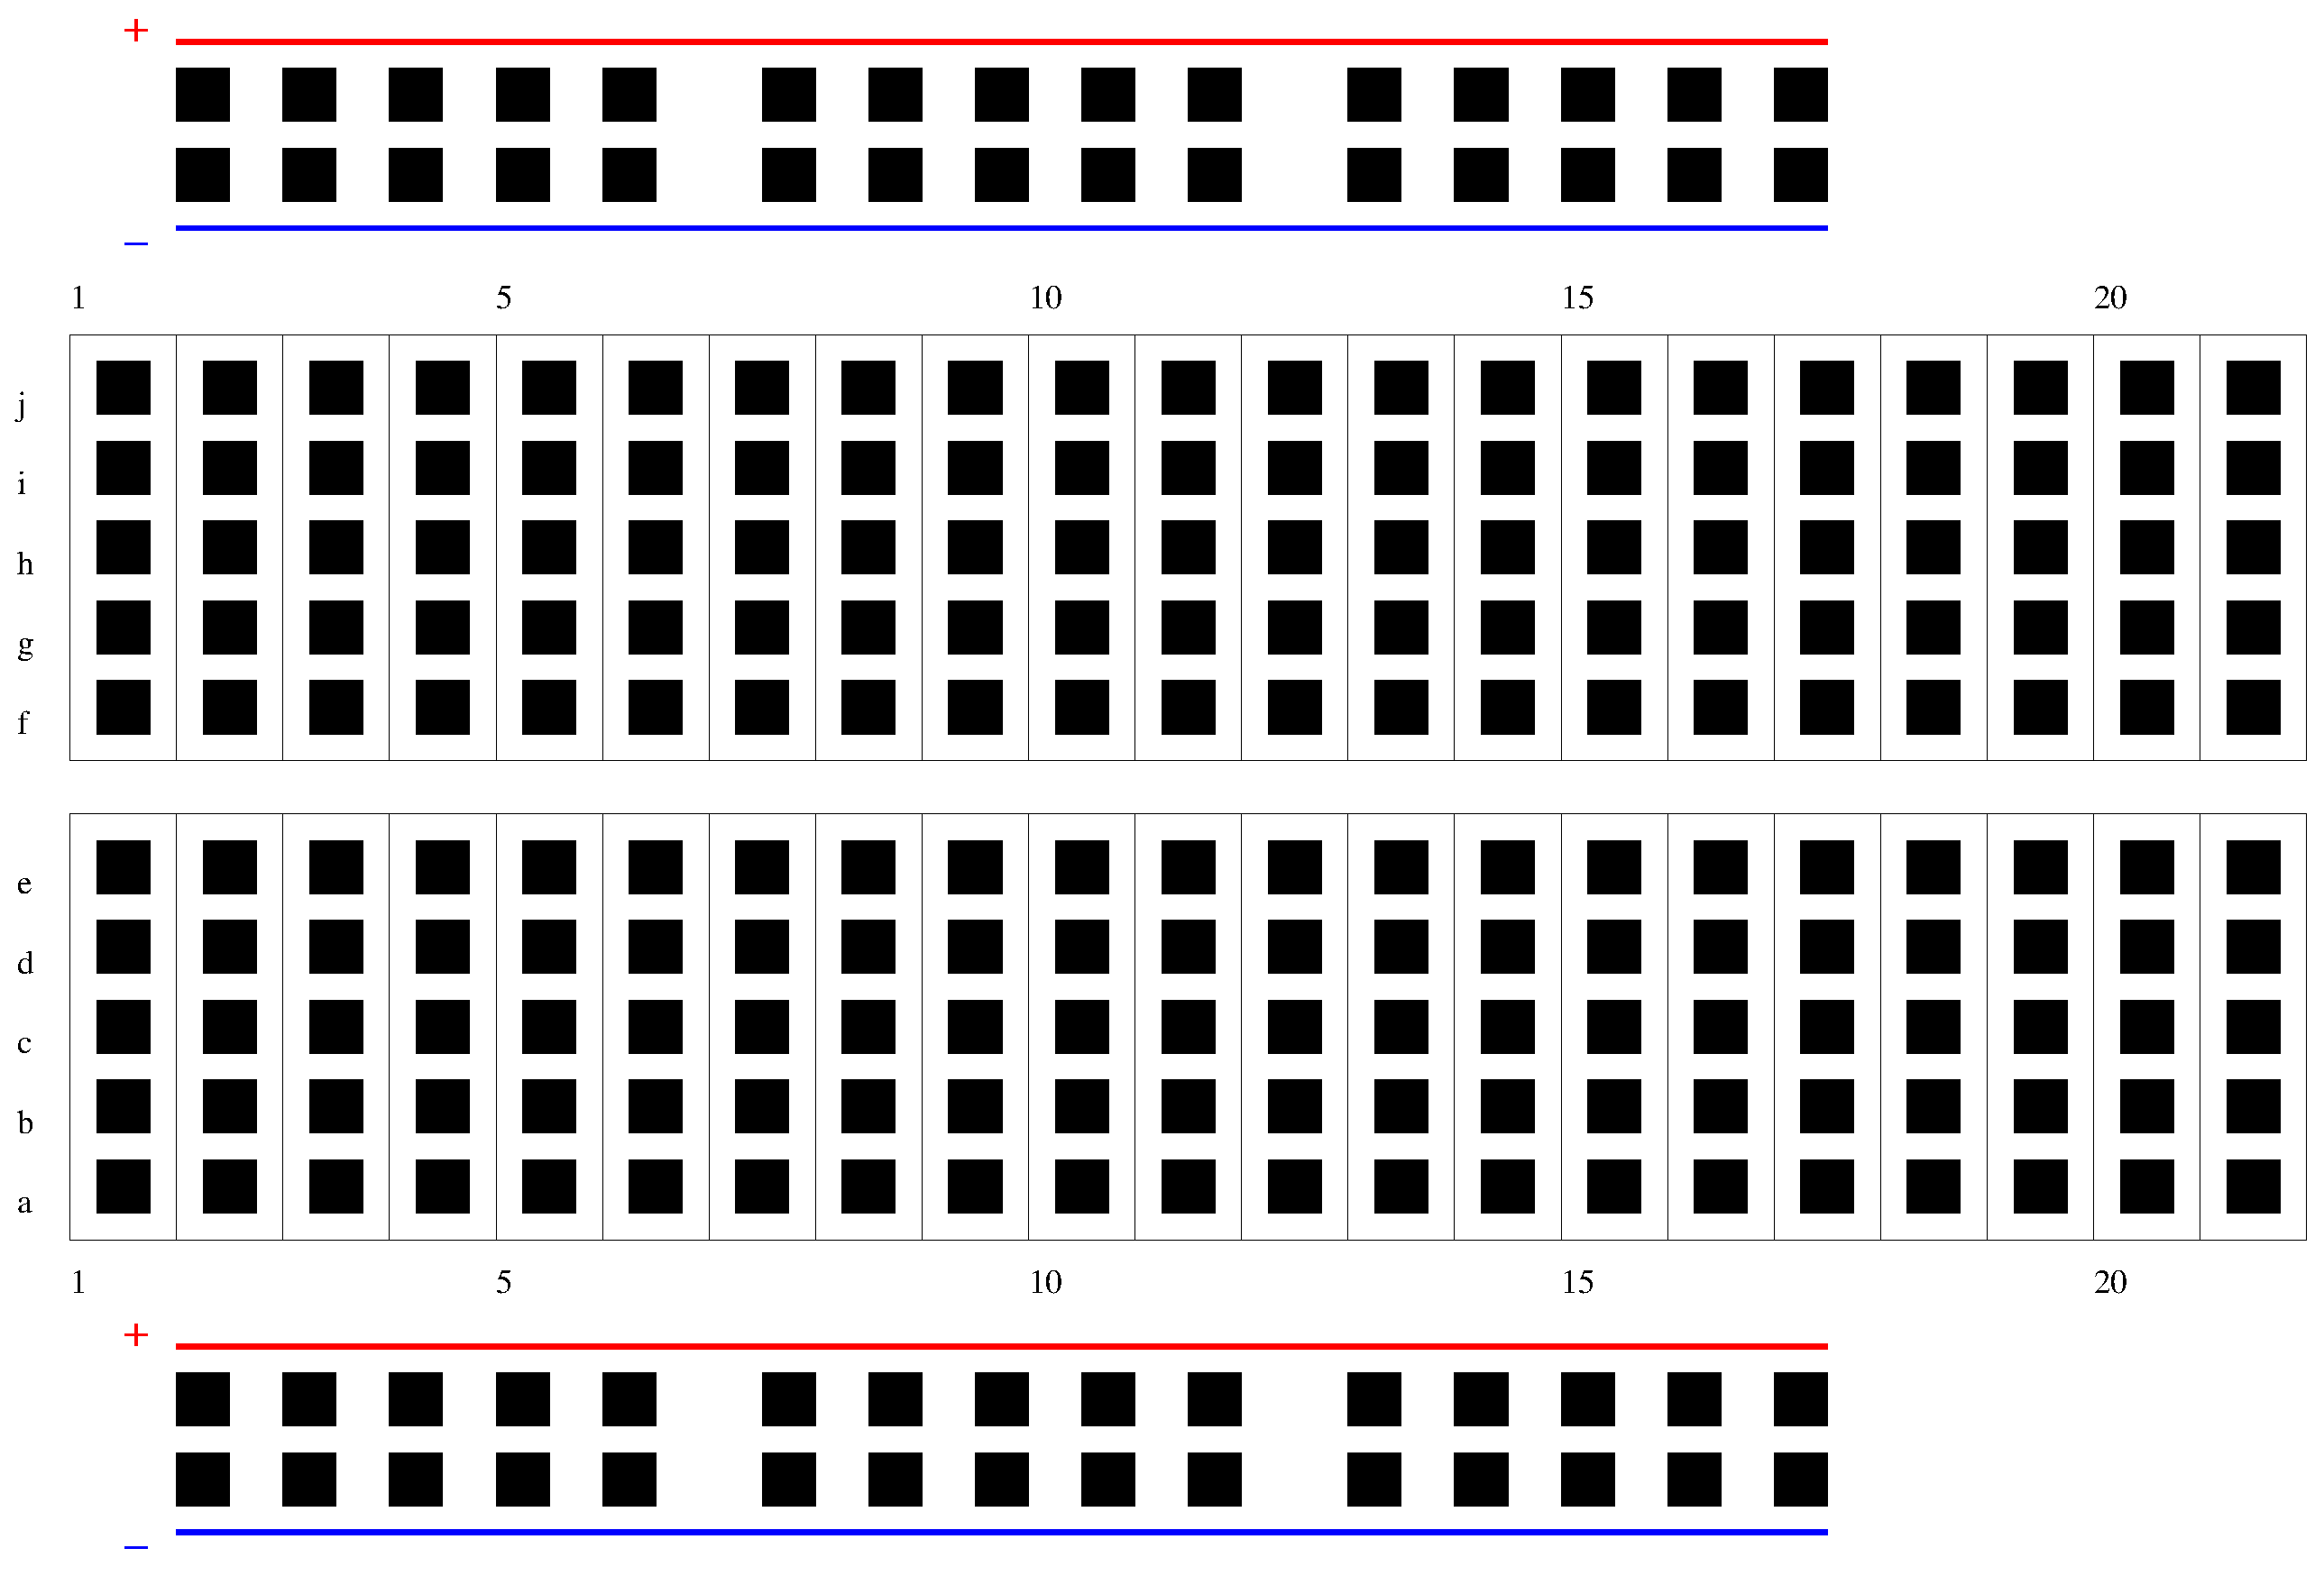
\includegraphics[width=0.7\linewidth]{figures/breadboard.eps}
  \caption{Breadboard
  \label{fig:breadboard}}
\end{figure}

Breadboards will help us to build circuits. It allows for effective connection between components without worrying about the electrical subtleties or hazards. Taking Figure~\ref{fig:breadboard} as a reference, the breadboard has internal electrical connections that makes it possible to tie multiple components to a single point. It does so by representing a \emph{physical} connection as multiple rows of the same column. That is: holes $1$a and $1$d are physically connected inside the breadboard's circuitry, whereas $3$d and $4$a are not.

Each breadboard is divided by thick spaces among different sections. In Figure~\ref{fig:breadboard}, there are four distinct sections: two with the $+$ and $-$ symbols, and two with numbers and letters. The latter was described above, whereas the former works in the opposite way: holes are connected with other holes in the same row. This section is often used to power the circuit, but more on that further in the practice.

Before writing any code, try to assemble the parts as shown in Figure~\ref{fig:blinkingLEDAdvancedLayout}.

\begin{figure}[htbp]
  \centering
  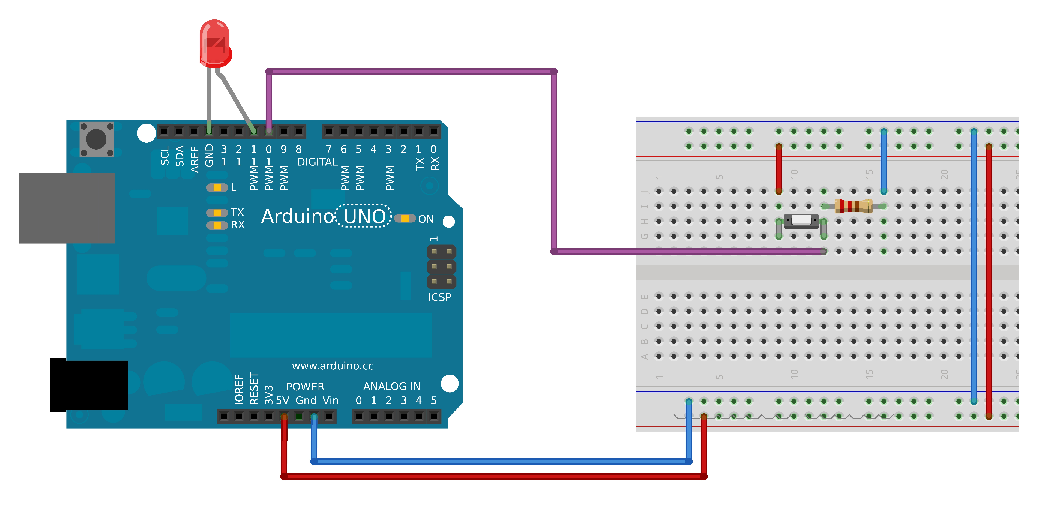
\includegraphics[width=0.9\linewidth]{figures/blinkingLEDAdvanced-NEW.eps}
  \caption{Blinking LED advanced layout
  \label{fig:blinkingLEDAdvancedLayout}}
\end{figure}

To avoid any confusion, let's review the layout component by component:

\begin{enumerate}
	\item Place the pushbutton on your breadboard. In Figure~\ref{fig:blinkingLEDAdvancedLayout}, the two pushbutton "legs" are inserted into holes $5$c and $6$c. In this example, the pushbutton will be energised through the $5$c leg.
	\item Connect one of the legs of the resistor to the negative leg of the pushbutton (hole $6$b). This will physically connect the resistor to one of the legs of the pushbutton. Insert the other leg on hole $9$b.
	\item In order to avoid confusion, cables on all figures are color coded. \emph{Red} represents power cables, \emph{blue} are connections to GND and \emph{cyan} are connections to IO pins on the Arduino. Try to duplicate the layout of Figure~\ref{fig:blinkingLEDAdvancedLayout}.
\end{enumerate}

Note that connecting the $+$ row to the Arduino's $5$V pin will provide $5$V to all the $+$ row. The same is true for GND and the $-$ row. This is very useful to avoid running out of $5$V of GND pins.


\subsection{The code}

Type the following instructions as a new file in the Arduino IDE:

\begin{lstlisting} [caption = {Blinking LED advanced example code}, language = C, label = {code:blinkingLEDAdvanced}, numbers = left, escapeinside={@}{@}]
// Turns on LED when pushbuttom is pressed and
// turns it off when pressed again.

const int LED = 11; @\label{BLA:LED}@
const int BUTTON = 10; @\label{BLA:BUTTON}@
int val = 0;@\label{BLA:val}@
int old_val = 0; @\label{BLA:old_val}@
int state = 0; @\label{BLA:state}@

void setup(){
	pinMode(LED, OUTPUT);@\label{BLA:pinModeLED}@
	pinMode(BUTTON, INPUT);@\label{BLA:pinModeBUTTON}@
}

void loop(){
	val = digitalRead(BUTTON);@\label{BLA:digitalRead}@
	
	//check if the button was pushed
	if((val = = HIGH) && (old_val = = LOW)){@\label{BLA:ifState}@
		state = 1 - state;
		delay(10); @\label{BLA:delay}@
	}@\label{BLA:endIfState}@
	
	old_val = val;@\label{BLA:old_valReasignment}@
	if(state = = 1){
		digitalWrite(LED, HIGH); @\label{BLA:turnOn}@
	}else{
		digitalWrite(LED, LOW);
	}
}
\end{lstlisting}

Let's review the code:

\begin{itemize}
	\item Line~\ref{BLA:LED}: sets the pin for the LED.
	\item Line~\ref{BLA:BUTTON}: assigns the input pin where the pushbutton is connected.
	\item Line~\ref{BLA:val}: \texttt{val} is the variable holding the state of the input pin corresponding to the pushbutton.
	\item Line~\ref{BLA:old_val}: \texttt{old\_val} holds \texttt{val}'s previous value.
	\item Line~\ref{BLA:state}: the variable \texttt{state} determines de condition of the LED. $0$ = off and $1$ = on.
	\item Line~\ref{BLA:pinModeLED}: the function \texttt{pinMode()} sets the roll of each pin. In this case, pin \texttt{LED} is set to \texttt{OUTPUT}.
	\item Line~\ref{BLA:pinModeBUTTON}: sets pin \texttt{BUTTON} to \texttt{INPUT}.
	\item Line~\ref{BLA:digitalRead}: asks whether there is any power at the specified pin. It returns HIGH or LOW if the button is being pushed or not, respectively.
	\item Line~\ref{BLA:ifState}: if the button is being pushed, then \texttt{val} = HIGH and \texttt{old\_val} = LOW. This provokes a change in \texttt{state}.
	\item Line~\ref{BLA:delay}: prevents errors in the change of \texttt{state}. Given that \texttt{loop()} repeats several hundred thousand times per second, making the processor wait a little bit allows for a correct reading of the pushbutton.
	\item Line~\ref{BLA:old_valReasignment}: the value of \texttt{val} is now old. Notice that once the LED is turned on, \texttt{val} = \texttt{old\_val} = LOW. Furthermore, \texttt{val} only changes when the button is pushed.
	\item Line~\ref{BLA:turnOn}: turn LED on.
\end{itemize}



%\chapter{An introduction to zigbee and 802.15.4}

\chapter{Introduction to XBee}\label{introToXBee}


One of the main characteristics of WSNs is the ability each node has to wirelessly communicate with other nodes. 
During this course we will be doing this with ZigBee protocol compliant radios, like XBee~\cite{faludi2010bws}.

Throughout this section you will be introduced to the different components and code that will allow you to set a basic wireless network with XBee modules.

\section{The Zigbee and IEEE 802.15.4 standards}

XBee is a Zigbee compliant hardware.
Zigbee is a specification that is build on top of IEEE 802.15.4.
Zigbee covers the upper layers of the protocol stack while IEEE 802.15.4 covers the lower layers (MAC and PHY).

ZigBee is intended for low-throughput, low-power, low-cost applications.For this reason, it is much simpler than other protocols such as WiFi (IEEE 802.11).
It has support for mesh topologies, which means that ZigBee devices relay messages for each other through multiple wireless hops.
The name ZigBee comes from the fact that the bees can dance to pass messages to each other, also in a multi-hop fashion.

There are channesl in the 868 MHz, 915 MHz and 2.4 GHz ISM bands and the speed is up to 250 kbps in the 2.4 GHz band.

Applications include domotics and wireless sensor and actuator networks.

\subsection{ZigBee profiles}
\begin{itemize}
\item ZigBee Co-ordinator: It is the most powerful device. There is a single coordinator in each network.
It is the node that creates the network and the other nodes simply join.
Quite often, this is the sink of the wireless sensor network that gathers all the data that is transmitted.
One of the co-ordination tasks is to assign short addresses as will be explained in the next subsection.
\item ZigBee Router: Routers are intermediate devices.
They can relay packets for other nodes.
They join a network that already exists and then announce it using beacons.
Therefore, they can have ``children'', nodes that join the network by establishing communication with the router.
\item End Devices:
These are the simplest devices.
They cannot forward packets; they cannot have children that depend on them and quite often they sleep to save energy.
\end{itemize}

\subsection{Network layer and addressing}

Addressing follows a hierarchical scheme that is explained in detail in \cite{baronti2007wsn}.
An example is provided in Fig. \ref{fig:hierarchical_addressing}

\begin{figure}[htbp]
  \centering
  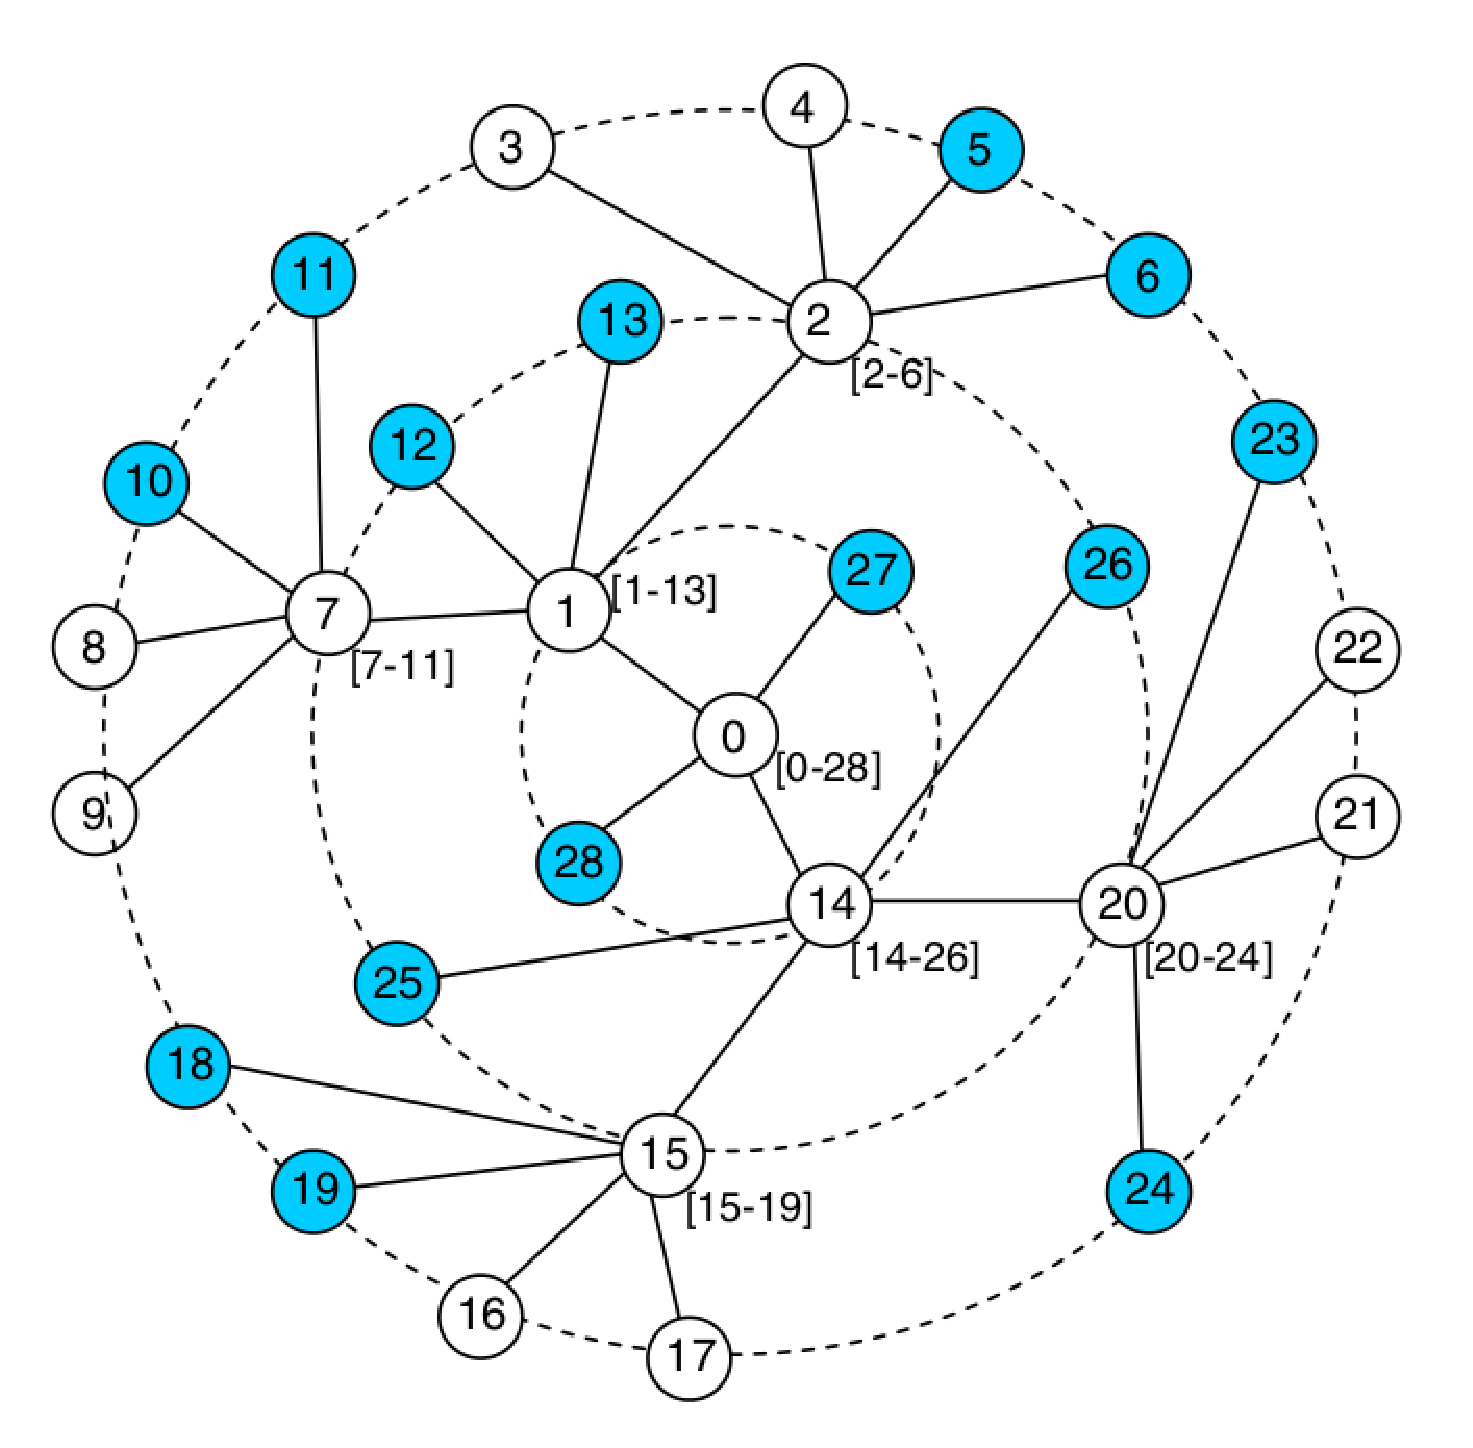
\includegraphics[width=0.4\linewidth]{figures/hierarchical_addressing.eps}
  \caption{Hierarchical address scheme in ZigBee (picture from \cite{baronti2007wsn})}
  \label{fig:hierarchical_addressing}
\end{figure}

The hierarchical scheme is appropriate for tree topologies and tree routing.
Three different topologies are supported in ZigBee: Star, tree and mesh.
They are shown in Fig. \ref{fig:zigbee-topologies}.

\begin{figure}[htbp]
  \centering
  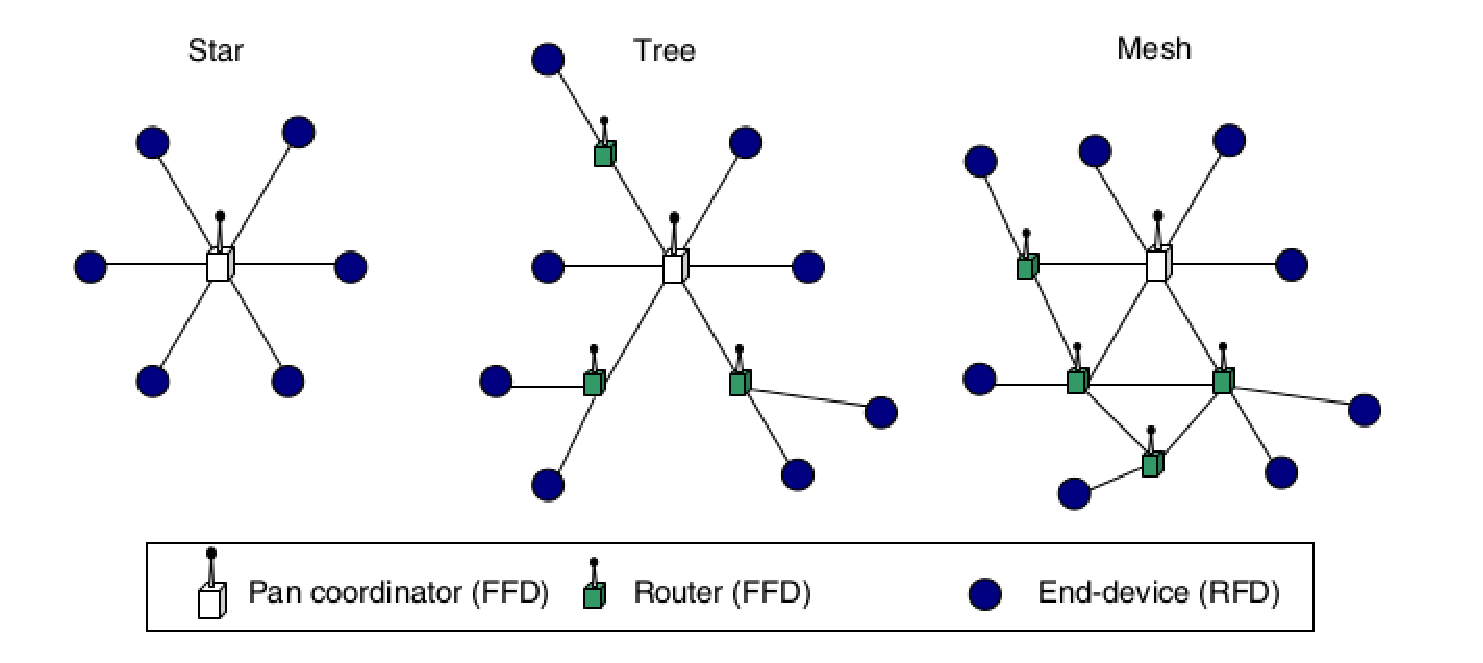
\includegraphics[width=0.6\linewidth]{figures/zigbee-topologies.eps}
  \caption{Supported topologies in ZigBee (picture from \cite{baronti2007wsn})}
  \label{fig:zigbee-topologies}
\end{figure}

The mesh topology requires a routing protocol and storing routing tables. 
It is very resource consuming and a device might not have the resources to execute it.
If a device does not have resources to launch a route discovery, it reverts to tree routing, which uses a trivial routing algorithm.
The flow chart is shown in Fig. \ref{fig:zigbee-flowchart}.

\begin{figure}[htbp]
  \centering
  \includegraphics[width=0.6\linewidth]{figures/zigbee-flowchart.eps}
  \caption{Routing a packet in ZigBee (picture from \cite{baronti2007wsn})}
  \label{fig:zigbee-flowchart}
\end{figure}

Another router alternative, when the sink is powerful and the other devices not so much, is source routing.
In source routing, when the sink sends a packet, it provides the full route that the packet has to follow.

In ZigBee, each node has two different addresses.
The serial number, or hardware address, which is a 64 bits address that is assigned at manufacturing time and is unique in the world.
Then there is the network address, which is only 16 bits, that is assigned by the network coordinator and is unique in the network.

There are some special addresses that are possible to highlight.
0x0000 0000 0000 0000 means that the destination is the coordinator.
0x0000 0000 0000 FFFF is for broadcast.
The short address 0xFFFE is used when the short address is not known or for broadcast.

When the short address is not known, the first step is an address resolution (from long address to short address).

Each network is identified by a ``Personal Area Network Identifier'' or PANId.
When we configure a network, we must ensure that all the devices are configured with the same PAN Id. 
And also be very careful in assigning different PAN Ids to different networks.
Specially in a classroom situation, if two teams use the same PAN Id, unexpected results may happen.


\section{The XBee module hardware configuration}\label{xbee:hardware}

XBee modules come in different configurations. The one we will be using is called XBee Series 2 with wire antenna as it is shown in Figure~\ref{fig:xbee}.

Other configurations include older versions, different antennas or connectors, different frequency band, and the ``pro'' version of XBee with higher transmission power and subsequent increase in coverage range and power consumption.


\begin{figure}[htbp]
  \centering
  
\includegraphics[width=0.4\linewidth]{figures/xbee.eps}
  \caption{XBee Series 2 with wire antenna
  \label{fig:xbee}}
\end{figure}

This device supports different kinds of ZigBee in mesh networking. Its wire antenna provides omnidirectional coverage, or what is the same as saying that its coverage is pretty much the same in all directions when the antenna is straight and perpendicular to the module.

If you flip the XBee, you will be able to see the pins through which it can send/receive data to/from sensors, communicate with Arduino, connection to a power supply and GND (more information about the pins can be found in page 15 of~\cite{faludi2010bws}).

\subsubsection{Preparing the XBee for configuration}

We can access and program the XBee through any terminal application and a USB connection. The \emph{breakout board} shown in Figure~\ref{fig:breakoutBoard} allows us to: $1$) plug the XBee into a breadboard, facilitating the wired connections with other components (including the Arduino); as well as the ability to $2$) establish a USB connection to configure the XBee.

\begin{figure}[htbp]
  \centering
  \includegraphics[width=0.4\linewidth]{figures/breakoutBoard.eps}
  \caption{XBee Explorer board from SparkFun
  \label{fig:breakoutBoard}}
\end{figure}

As the pins on the XBee are separated differently than the holes in the breadboard, every time a configuration or wired connection is needed, the XBee should be placed in the breakout board as shown in Figure~\ref{fig:xbeeAndBreakoutBoard}, and then placed on the breadboard.

\begin{figure}[htbp]
  \begin{center}$
    \begin{array}{cc}
      \includegraphics[width=0.4\linewidth]{figures/xbeeAndBreakoutBoard.eps}\label{xbeeOutside} &
      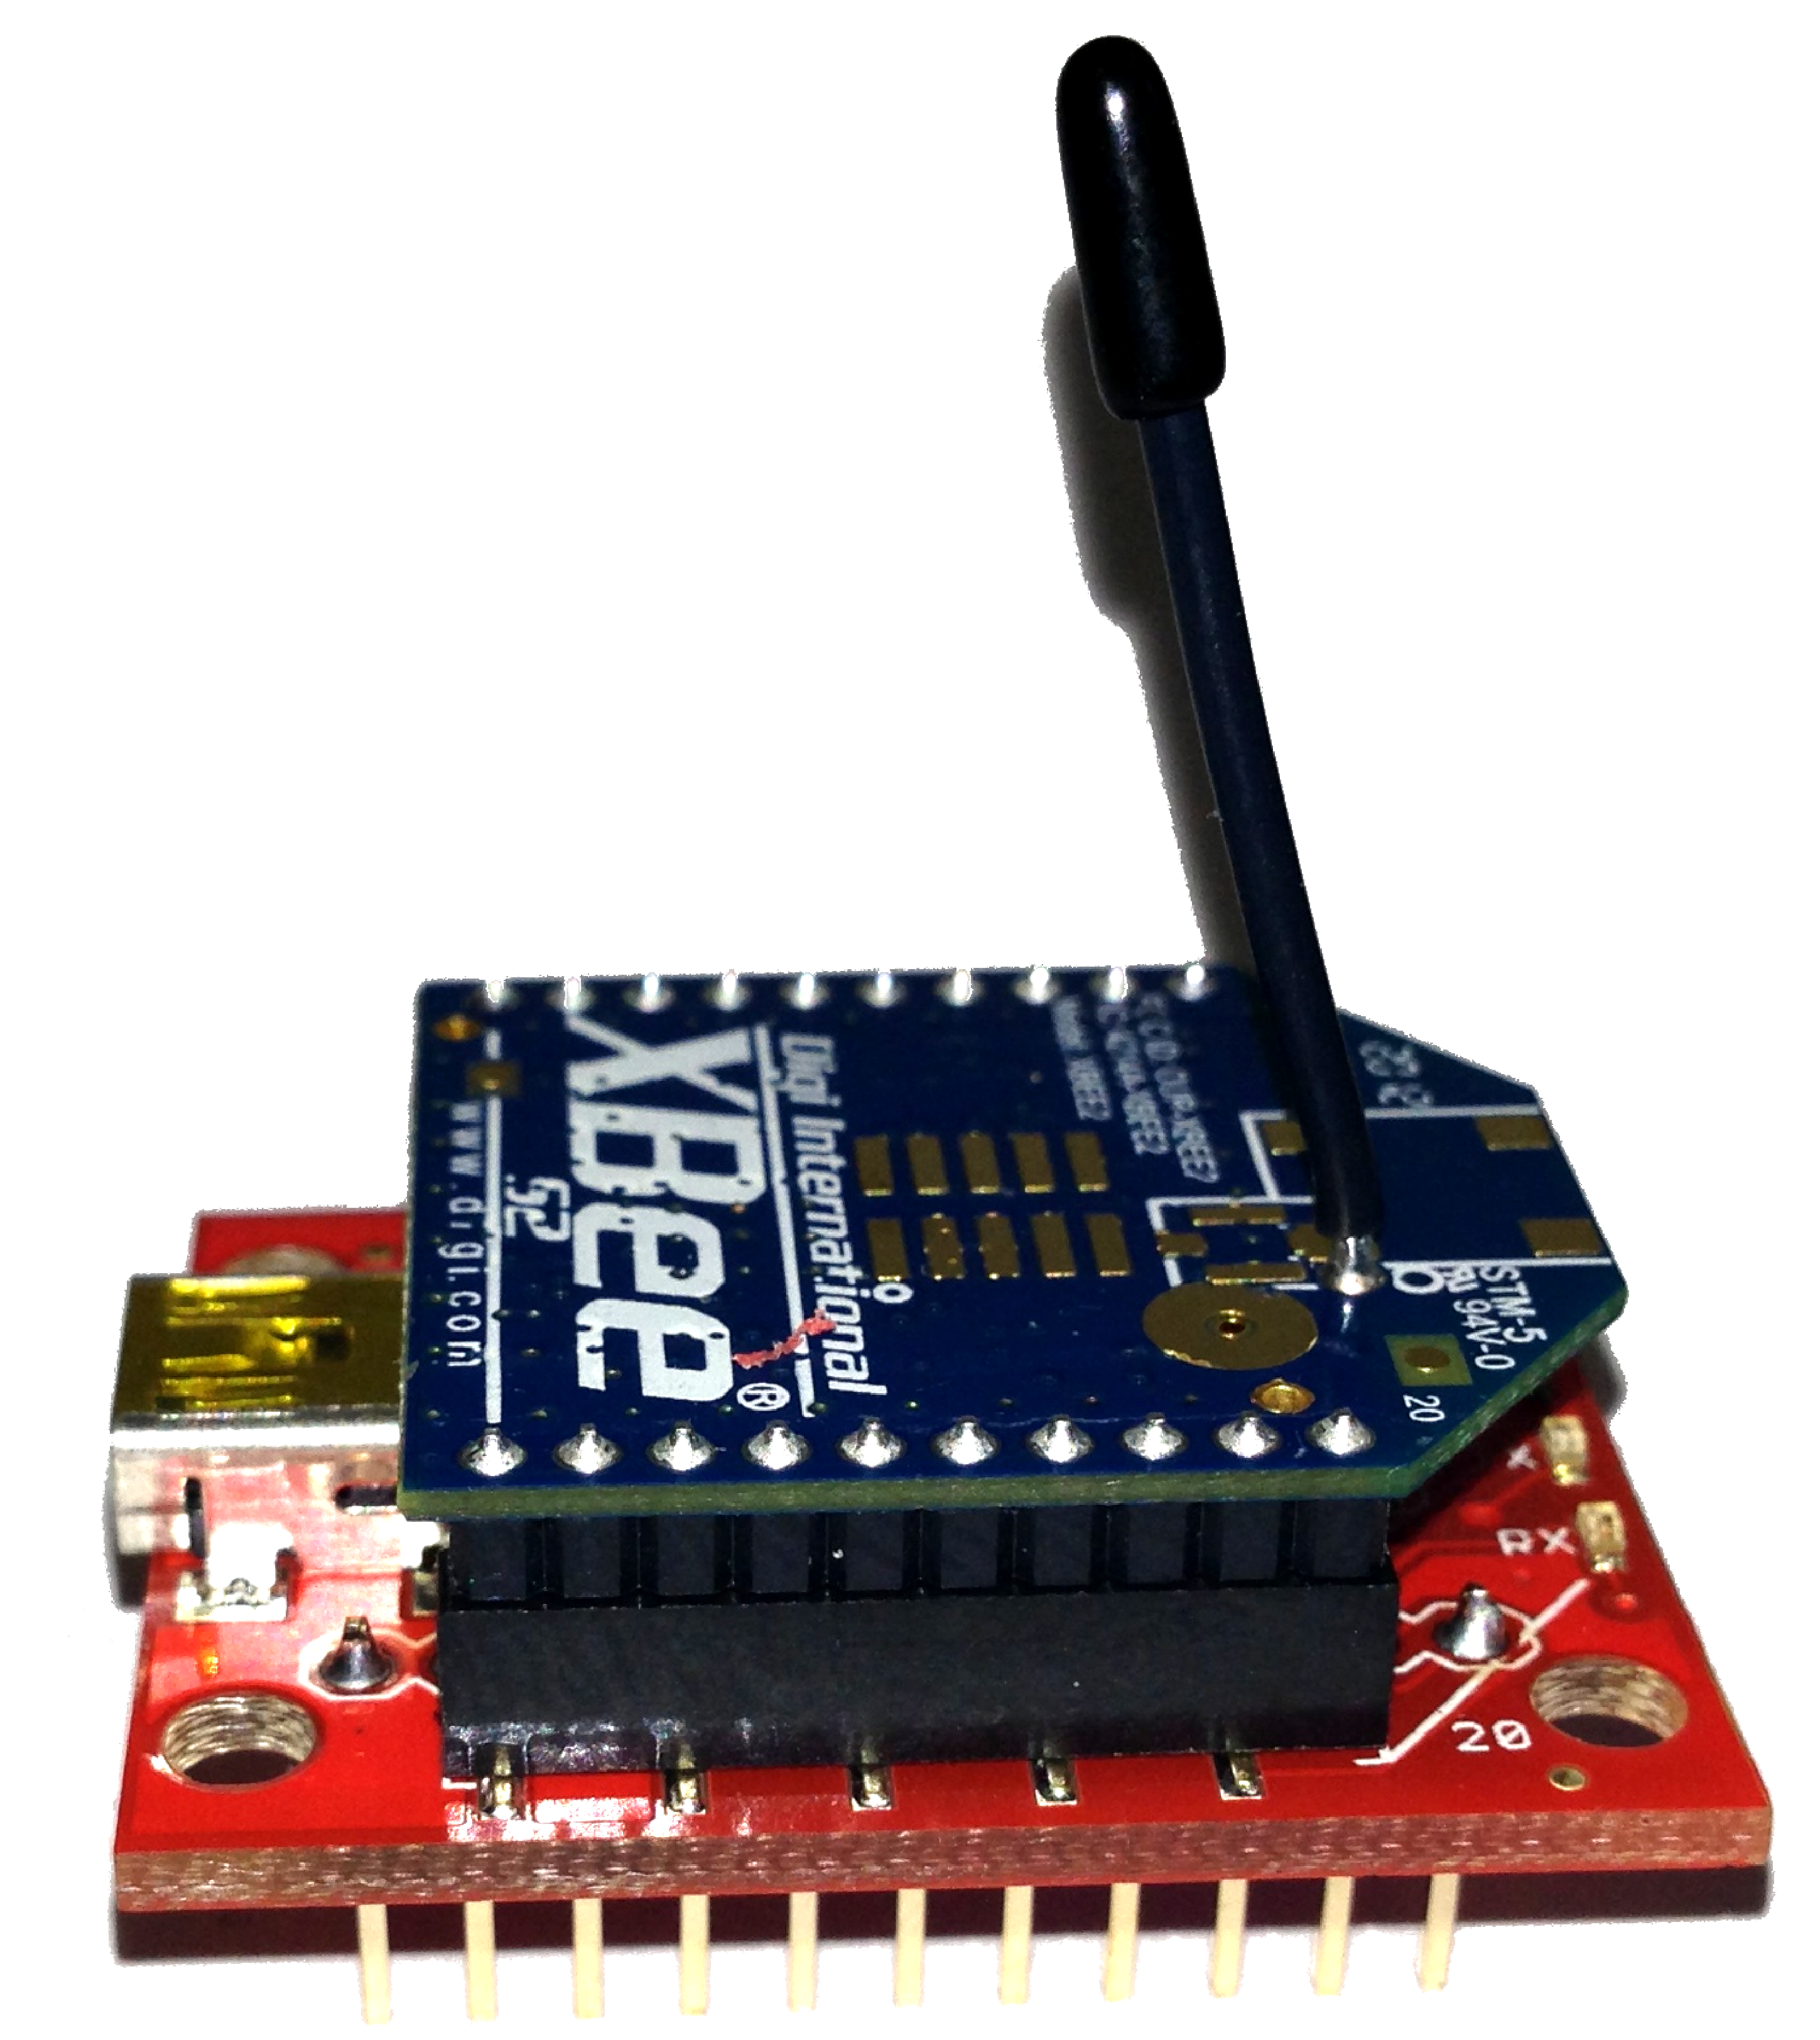
\includegraphics[width=0.4\linewidth]{figures/xbeeAndBreakoutBoard-inserted.eps}\label{xbeeInside}
    \end{array}$
  \end{center}
  \caption{XBee and breakout board: Left: XBee outside; see the different spacing of the pings. Right: XBee inside; setup for configuring and pluging into breadboard.
    \label{fig:xbeeAndBreakoutBoard}}
\end{figure}

It is important to notice that once the XBee is placed on the breakout board, the pins functions change. The new role of each pin is now the displayed underneath the breakout board, as in Figure~\ref{fig:xbeeBreakoutBoardPins}.

\begin{figure}[htbp]
  \centering
  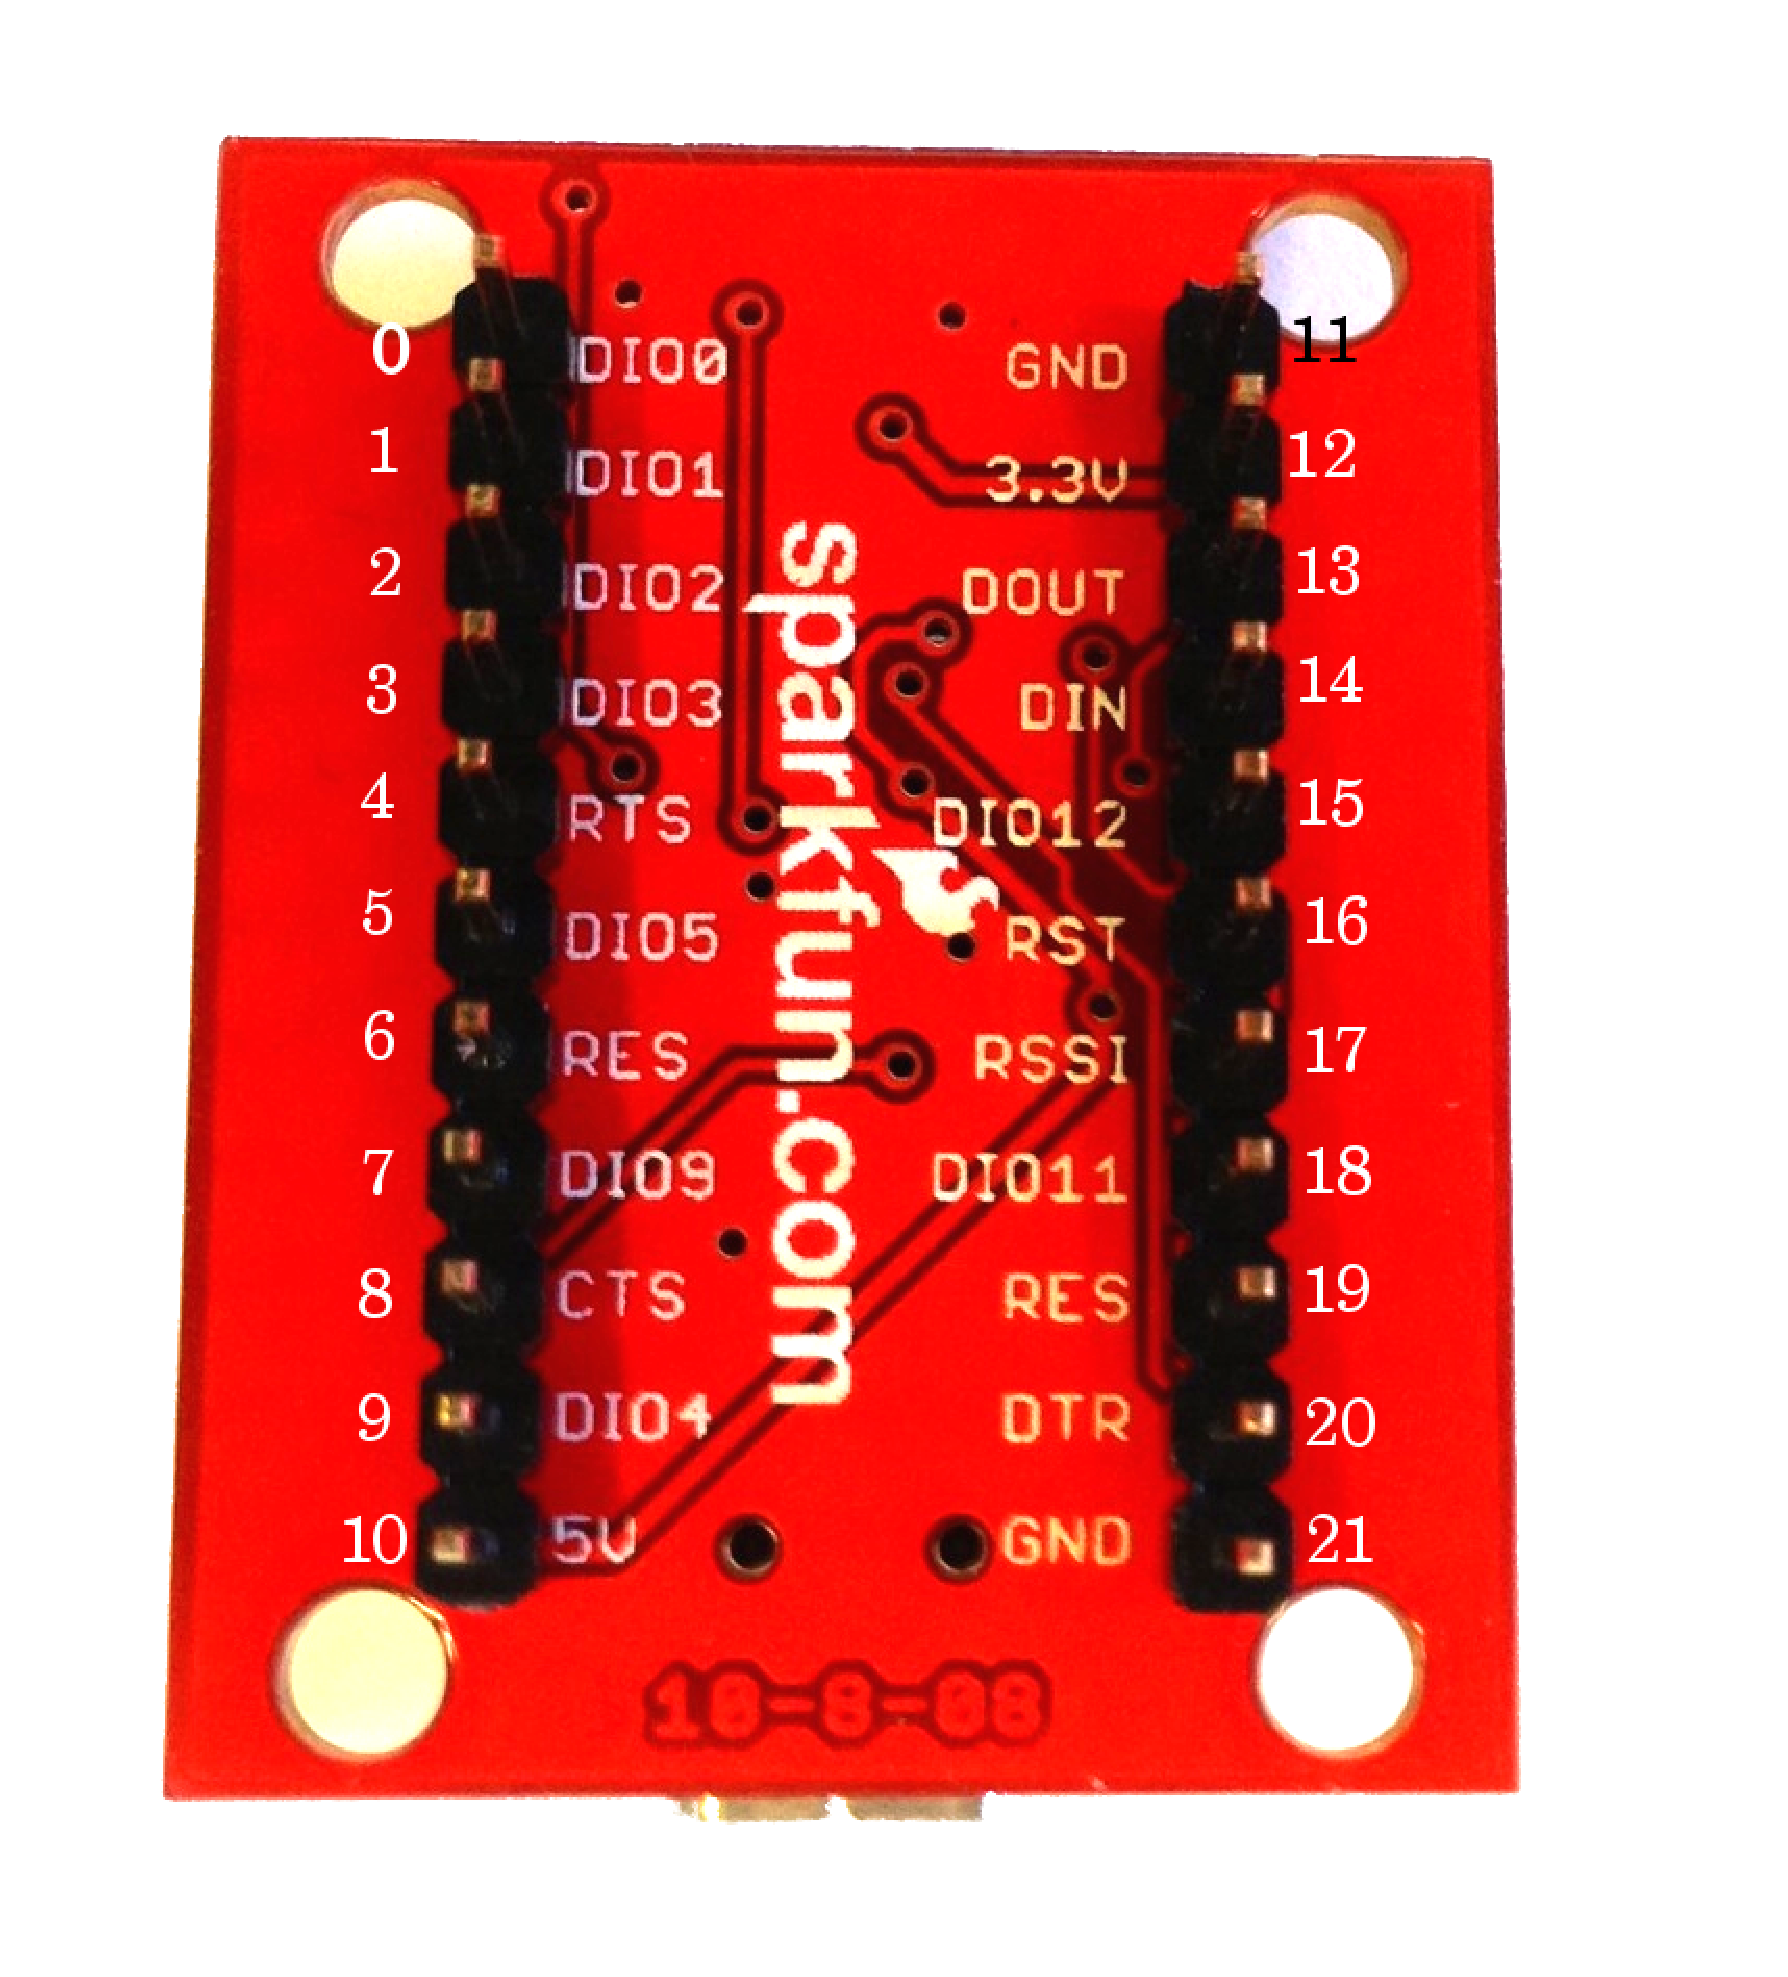
\includegraphics[width=0.6\linewidth]{figures/xbeeBreakoutBoardPins.eps}
  \caption{XBee Explorer pins
  \label{fig:xbeeBreakoutBoardPins}}
\end{figure}

There are some pins that have additional functionalities.
As an example, the pin labeled DIO5 is also the association pin.
It is high when the XBee is looking for a network and blinks when it associates to a network (PAN).

The Explorer board also have some useful LEDs.
The PWR LED tells us that it is powered.
TX and RX blink when we have serial transmission and reception.
RSSI lights up for ten seconds after wireless transmission or reception.

Now that the device is properly placed, we need to setup a connection so the current configuration can be reviewed and changed.

\subsubsection{Accessing the firmware}\label{xbeeRoleConfiguration}

The XBee has a microcontroller running a configurable firmware. This firmware holds the necessary information for addressing, communication, security and utility functions. You can configure this firmware to change different settings like: local address, security settings, destination address and how the analog sensors connected to its pins are read.

As for now, the official way to update this firmware is through a program called \emph{X-CTU} and can be downloaded for free from the \emph{\color{blue}{\href{http://www.digi.com/support/kbase/kbaseresultdetl?id=2125}{XBee manufacturer's website}}}.

\emph{\color{blue}{\href{http://www.digi.com/support/productdetail?pid=4549&osvid=0&type=firmware}{Firmware updates}}}

X-CTU is only available for the Microsoft Windows operating system, nevertheless you have the virtualization option in OS X, as well as WINE Windows emulator in Linux. 
If you choose WINE to run X-CTU, it is necessary to add a virtual link in the file system.
For example, a link from

\texttt{/home/jbarcelo/.wine/dosdevices/com5} 

to

\texttt{/dev/ttyUSB0}

It is also important to know that the user must be added to the \texttt{dialout} group.
And the firmware for the XBee must be downloaded manually.
Then use the button ``Download new versions ... '' in the ``Modem Configuration'' tab.
Then choose ``File'' for the upload source.

To take a peek at the current XBee configuration: 

\begin{enumerate}
	\item Plug it into one of your computer's USB ports and launch the X-CTU application.
	\item Select the appropriate Com Port listed under \emph{Select Com Port}. This port should be the same in which your XBee is connected.
	\item Confirm that everything is setup correctly by clicking on the \emph{Test/Query} button. If everything is alright, a pop-up window will display the modem type and firmware version.
	\item Change to the \emph{Modem Configuration} tab on the top the X-CTU window. This tab will show you how the firmware is configured.
	\item Under \emph{Modem Parameters and Firmware}, click on the \emph{Read} button. This will fill the current window with the current firmware configuration, as well as the XBee's \emph{Modem} and \emph{Function Set}.
\end{enumerate}

Luckily, X-CTU is only required for upgrading the firmware. For changing the XBee's configuration we only need a USB connection and a terminal software. Nevertheless, this is only possible if the XBee is on \emph{AT command mode} (capable of receiving human commands and forward messages without performing any modification, see Table~\ref{tab:xbeeATModes}). To set it on, follow these steps:

\begin{enumerate}
	\item In the \emph{Model Configuration} tab of the X-CTU, check that the \emph{Modem type} is set to \texttt{XB24-ZB}.
	\item To start, we are going to configure two XBee radios. Under \emph{Function Set}, choose \texttt{ZIGBEE COORDINATOR AT}.
	\item Choose any version greater than \texttt{0x2070}.
	\item Click on the \emph{Write} button to program this device as a coordinator.
\end{enumerate}

Once the installation is complete, gently remove the USB from the first XBee radio a plug it into another. Repeat the process described above, but now under \emph{Function Set} choose \texttt{ZIGBEE ROUTER AT}. Select the highest version available and click on \emph{Write} to program the device.

It is important to distinguish between the two XBee you just configured, given that they behave differently. Every ZigBee network must contain only one coordinator radio, this way the network can be properly defined and managed. Mark which configuration each radio has with a sticker to eliminate any confusion.

\begin{table}[htbp]
	\centering
	\caption{XBee AT modes}
	\label{tab:xbeeATModes}
	\scalebox{0.7}{
	\begin{tabular}{c||c}
		\hline
		\bfseries Transparent mode & \bfseries Command mode\\
		\hline\hline
		Talk \emph{through} the XBee & Talk \emph{to} the XBee itself\\
		Any data can me sent through & Only responds to AT commands\\
		Default state & {\bfseries +++} to enter mode\\
		Wait $10$ seconds to return to this mode & Times out after 10 seconds of no input\\
		\hline
	\end{tabular}}
\end{table}

\subsubsection{Configuring the XBee through a terminal }

There are a lot of terminal applications. Fortunately, most of them need the same kind of information to establish a connection through USB. Table~\ref{tab:terminalParameters} gathers the required settings for a serial terminal software attempting to establish a connection with the XBee.

\begin{table}[htbp]
	\centering
	\caption{Default terminal settings for establishing a connection with an XBee}
	\label{tab:terminalParameters}
	\scalebox{0.7}{
	\begin{tabular}{c||c}
		\hline
		\bfseries Setting & \bfseries Value\\
		\hline\hline
		Baud & $9600$\\
		Data & $8$~bit\\
		Parity & None\\
		Stop bits & $1$\\
		Flow control & None\\
		Line feed & CR+LF or Auto Line Feed\\
		Local echo & on\\
		\hline
	\end{tabular}}
\end{table}

To check if you are already inside the XBee, try asking the radio to go to command mode issuing the \texttt{+++} instruction. If after a moment an \texttt{OK} appears at the right hand side, then you are in!

\subsubsection{Reviewing some AT commands for the XBee}

Issuing commands from a serial connection (like the one you established with the terminal program) to the XBee follows a simple guideline: \emph{instruction parameter} \texttt{<CR>}. Where \texttt{<CR>} accounts for \emph{carriage return}, and just means that you have to press the Return (Enter) key to submit the command. Passing and empty \emph{parameter} just outputs the current value of the specified register (the \emph{instruction} part of the command).

All AT commands start with the \texttt{AT} prefix (accounting for \emph{attention}) and then are followed by a two letter character command identification. Some of the basic AT commands are described below, as well as in~\cite{faludi2010bws}.

\begin{itemize}
	\item \texttt{AT}: gets the attention of the XBee. Its normal output is \texttt{OK}. If you do not receive this output,  you've probably timed out of command mode and need to reissue the \texttt{+++} command to get back in it.
	\item \texttt{ATID}: without any parameter it shows the current Personal Area Network ID (PAN ID) that is assigned to the radio. You can set a PAN ID passing an hexadecimal number in the range $0$x$0$-$0$xFFFF as a parameter.
	\item \texttt{ATSH/ATSL}: it shows the \emph{high} or \emph{low} parts of the unique XBee $64$-bit serial number, respectively. This number cannot be changed, so passing a parameter will produce an \texttt{ERROR} response.
	\item \texttt{ATDH/ATDL}: it shows the \emph{high} or \emph{low} parts of the \underline{destination} address the local radio will forward messages to, respectively. Putting address information after \texttt{ATDH} or \texttt{ATDL} will set the \emph{high} or \emph{low} parts of the destination address, accordingly.
	\item \texttt{ATWR}: saves the current configuration to firmware, so it will become the default configuration the next time you power on the XBee.
    \item \texttt{ATCN}: leave command mode and activate transparent mode. You can also wait for 10 seconds to obtain the same result.
    \item \texttt{ATMY}: 16 bit address. It can only be read. It cannot be set.
\end{itemize}

		

	\section{Practice: Simple chat with XBee}\label{pract:simpleChat}

WSNs are composed of nodes able to send messages among themselves. In this practice you will be guided through the configuration of (at least) two XBees to build a basic chat application. Furthermore, you will have the opportunity to familiarize yourself with the XBee and the different AT commands described in Chapter~\ref{introToXBee}.

You will need:

\begin{itemize}
	\item One XBee Series 2 configured as a \texttt{ZIGBEE COORDINATOR AT}.
	\item One XBee Series 2 configured as a \texttt{ZIGBEE ROUTER AT}.
	\item As many breakout boards and USB cable A to mini B as XBee radios.
	\item One computer per XBee. It is less confusing than establishing multiple terminal sessions from one computer.
\end{itemize}

We need to be able to distinguish the coordinator radio from the router radios. It is easier if you write this addresses down. Proceed as follows:

\begin{enumerate}
	\item Establish a terminal connection to the coordinator radio.
	\item Once inside, issue the \texttt{+++} to enter to command mode.
	\item Type \texttt{ATSL} to reveal the lower part of the XBee serial number.
	\item Write it down: {\bfseries Coordinator address:} $0013$A$200$ \underline{\ \ \ \ \ \ \ \ \ \ \ \ }
\end{enumerate}

Repeat the same for the router AT.

{\bfseries Router address:} $0013$A$200$ \underline{\ \ \ \ \ \ \ \ \ \ \ \ }

Now, let's configure the coordinator.

\subsection{The code: coordinator}

The settings for the coordinator are contained in Table~\ref{tab:xbeeChatCoordinator} below.

\begin{table}[htbp]
	\centering
	\caption{XBee coordinator settings for simple chat}
	\label{tab:xbeeChatCoordinator}
	\scalebox{0.7}{
	\begin{tabular}{c||c||c}
		\hline
		\bfseries Description & \bfseries Command & \bfseries Parameter\\
		\hline\hline
		PAN ID & \texttt{ATID} & {\bfseries 2013}\\
		Destination address \emph{high} & \texttt{ATDH} & {\bfseries 0013A200}\\
		Destination address \emph{low} & \texttt{ATDL} & {\bfseries\underline{\ \ \ \ \ \ \ \ \ \ \ \ }}\\
		\hline
	\end{tabular}}
\end{table}

Note that the \emph{Destination address low} specified in Table~\ref{tab:xbeeChatCoordinator} correspond to the \underline{router} radio.

Issuing the commands on the terminal window will look like the listing below.

\begin{lstlisting} [caption = {Coordinator settings as seen in the terminal}, label = {code:xbeeChatCoordinator}, numbers = left, escapeinside={@}{@}]
+++
OK
ATID 2013
OK@\label{SC:instructionOK}@
ATDH 0013A300
OK
ATDL ____ //put the lower part of the router address
OK
ATID
2013
ATDH
0013A300
ATDL
____
ATWR
OK@\label{SC:writeOK}@
\end{lstlisting}

You will receive an \texttt{OK} after issuing a command (as in Line~\ref{SC:instructionOK}) as well as when writing to the firmware (Line~\ref{SC:writeOK}).

\subsection{The code: router}

The settings for the router must contain the same information collected for the coordinator. Fill out Table~\ref{tab:xbeeChatRouter} accordingly.

\begin{table}[htbp]
	\centering
	\caption{XBee router settings for simple chat}
	\label{tab:xbeeChatRouter}
	\scalebox{0.7}{
	\begin{tabular}{c||c||c}
		\hline
		\bfseries Description & \bfseries Command & \bfseries Parameter\\
		\hline\hline
		PAN ID & \texttt{ATID} & {\bfseries 2013}\\
		Destination address \emph{high} & \texttt{ATDH} & {\bfseries 0013A200}\\
		Destination address \emph{low} & \texttt{ATDL} & {\bfseries\underline{\ \ \ \ \ \ \ \ \ \ \ \ }}\\
		\hline
	\end{tabular}}
\end{table}

Note that the \emph{Destination address low} specified in Table~\ref{tab:xbeeChatRouter} correspond to the \underline{coordinator} radio.

\subsubsection{Chat!}
Now you just have to connect each XBee to one computer and establish a terminal connection to each one (or connect the two radios to the same computer running two different terminal applications, one for each XBee). Make sure all the connection settings are as specified in Table~\ref{tab:terminalParameters}, so you will not have any problems.

If both radios are in transparent mode (see Table~\ref{tab:xbeeATModes}), everything you type in one terminal will be forwarded to the other XBee.
	\chapter{Practice: Wireless doorbell}\label{pract:wirelessDoorbell}
\section*{Suggested read: Chapters~\ref{introToXBee} and~\ref{pract:simpleChat}}

This practice guides you through the construction of a wireless doorbell system. It is composed by two components: the switch and the buzzer.

On the switch side, we will be prototyping a layout like the one shown in Figure~\ref{fig:wirelessDoorbellSwitch}. While the sound will be produced by a buzzer on the other radio, like in Figure~\ref{fig:wirelessDoorbellBuzzer}.

You will need:

\begin{itemize}
  \item Eventhough the two components may fit in one breadboard; to make it more real, it is better to use two separate breadboards.
  \item Hookup wire. It is recommended to have at least four different colors.
  \item Two Arduino boards.
  \item USB A-to-B cable for the Arduinos.
  \item One $10$K resistor.
  \item One momentary switch or pushbutton for input.
  \item One buzzer for output.
  \item One XBee radio configured as \texttt{ZIGBEE COORDINATOR AT}.
  \item One XBee radio configured as \texttt{ZIGBEE ROUTER AT}.
  \item Two breakout boards.
  \item USB cable for the XBee breakout board.
\end{itemize}

Every ZigBee network has only one coordinator. Other nodes can be configured as routers. To configure your XBee radios, please refer to Chapter~\ref{xbeeRoleConfiguration}.

It is strongly suggested that you mark down the XBees to distinguish the coordinator from the router(s).

\section{Wireless doorbell connections layout}

\subsection{Switch}
Follow these guidelines to prepare the connections for the switch that will make the doorbell ring (or buzz in our case). If lost, you can always take a look at the final layout in Figure~\ref{fig:wirelessDoorbellSwitch}.

\begin{enumerate}
  \item Energize the breadboard by hooking up a {\color{red}{red}} wire from the Arduino $3.3$V output to one of the power rails of the breadboard.
  \item Hook up a {\color{blue}{blue}} wire from the ground (GND) connection on the Arduino to the ground rail on the breadboard.
  \item Place the XBee/breakout board with both sides on different sections of the breadboard, in a way that the space separating the sections passes under the XBee/breakout board.
  \item Use a {\color{red}{red}} wire to connect pin $3.3$V (or pin $1$ as in Figure~\ref{fig:xbeeBreakoutBoardPins}) of the XBee to the power rail on the breadboard.
\end{enumerate}


\begin{figure}[htbp]
  \centering
  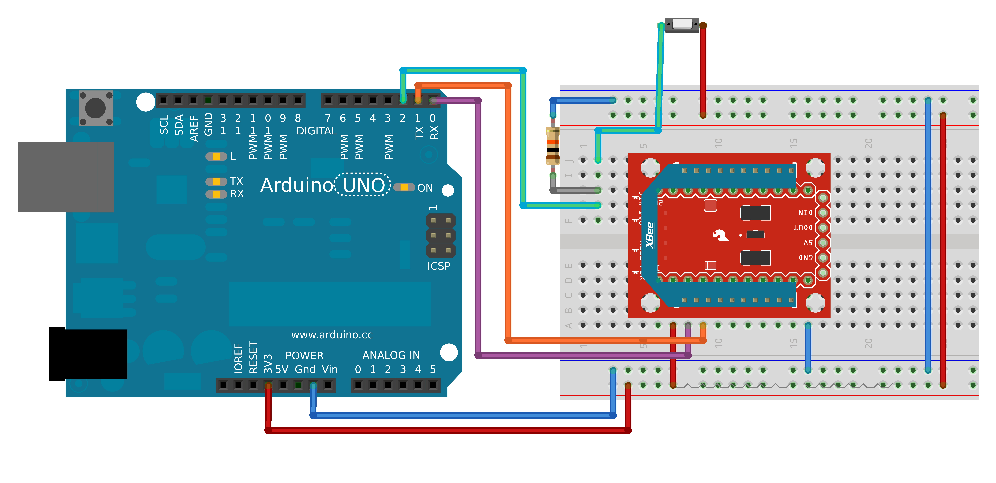
\includegraphics[width=\linewidth]{figures/doorbellSwitch-NEW.eps}
  \caption{Wireless doorbell: switch layout
  \label{fig:wirelessDoorbellSwitch}}
\end{figure}

\begin{figure}[htbp]
  \centering
  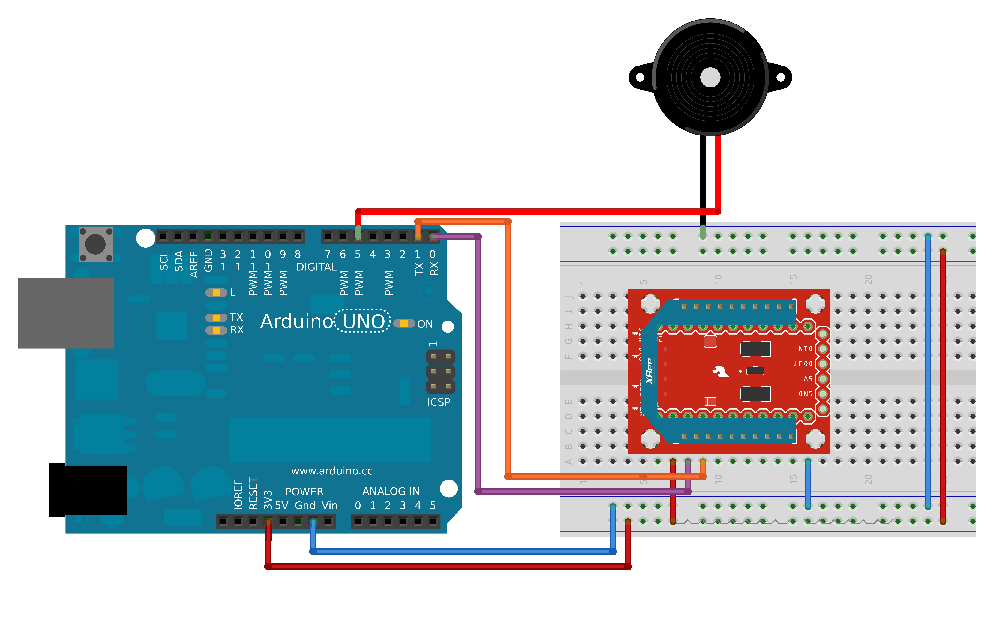
\includegraphics[width=\linewidth]{figures/doorbellBuzzer-NEW.eps}
  \caption{Wireless doorbell: buzzer layout
  \label{fig:wirelessDoorbellBuzzer}}
\end{figure}

\chapter{Practice: A WSN with XBee's AT mode}\label{ATSensorNetwork}
\section*{Suggested read: Chapers~\ref{introToXBee},~\ref{pract:simpleChat} and~\ref{pract:thermometer}}

In this assignment we will build a sensor network using the AT (as opposed to the API) mode.
This means that we will directly write characters in one end and read them at the other end.
We can replace any of the two ends by a serial terminal emulation (\emph{\color{blue}{\href{http://en.wikipedia.org/wiki/Minicom}{minicom}}}).

We start by flashing two XBees using X-CTU.
We will install the AT firmware in them.
One has to be the coordinator and the other the router.

Then we have to configure the PANID, and the destination address for each of them.
The configuration can be done using X-CTU or the minicom.
Verify the configuration observing the RSSI LED and then connecting minicom to both XBee and sending information from one XBee to the other as in the chat assignment (see Chapter~\ref{pract:simpleChat}).

We will use one of the XBees on the solderless breadboard, connected to the Arduino.
As usual, use the Arduino 3.3V to power the breadboard and connect the serial pins of the XBee to the Arduino.
Use the breadboard to install your light or temperature sensors and connect them to the analog inputs of the Arduino. You can take a look at Chapter~\ref{pract:thermometer} to ease your way through this task. Figure~\ref{fig:thermometerInArduino} provides the necessary connections.

\begin{figure}[htbp]
  \centering
  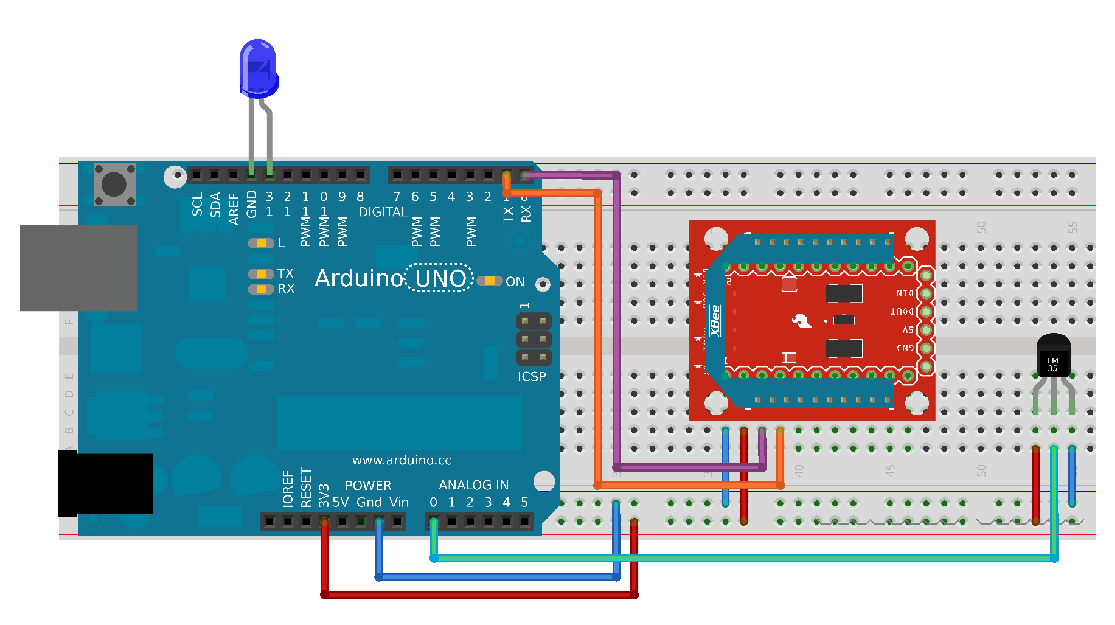
\includegraphics[width=0.85\linewidth]{figures/thermometerInArduino.eps}
  \caption{Thermometer and XBee transmitter.}
  \label{fig:thermometerInArduino}
\end{figure}

Use the example code in Listing \ref{code:ATWSN-router} as a reference to read data from the sensors and send it using the serial connection from the Arduino to the XBee. 
Then the XBee will automatically send it to the remote XBee.
Note that in the code we include identifiers for the node and sensor.

\begin{lstlisting} [caption = {Reading from analog input and sending the data via the XBee.}, language = C, label = {code:ATWSN-router}, numbers = left, escapeinside={@}{@}]
int ledPin = 13;

void setup()
{
  pinMode(ledPin, OUTPUT);
  Serial.begin(9600);
}

void loop()
{
  digitalWrite(ledPin, HIGH);
  delay(1000);
  digitalWrite(ledPin, LOW);
  delay(1000);
  Serial.print("N "); //node
  Serial.print("10 ");
  Serial.print("S "); //sensor
  Serial.print("1 ");
  Serial.print("T ");
  Serial.println(analogRead(A0));
}
\end{lstlisting}


The other XBee will be connected directly to the computer.
This will be the sink and will gather the sensed data.
We will program this part in Python using the Listing \ref{code:ATWSN-sink} for reference.


\begin{lstlisting} [caption = {Simple code that reads the message that arrive to the XBee in AT mode.}, language = Python, label = {code:ATWSN-sink}, numbers = left, escapeinside={@}{@}]

# Derived from code by Alejandro Andreu
import serial
import time
import sys
import shlex
from time import gmtime, strftime

print 'Receiving data in transparent mode'

def main():
    if len(sys.argv) is 1:
        print 'You must provide the path to the serial port as an argument, for instance: "python <code.py> /dev/ttyUSB0".'
        sys.exit()
    portname = sys.argv[1]
    try:
        with open(portname) as f: pass
    except IOError as e:
        print e, '\n'
        sys.exit()

    s = serial.Serial(portname, 9600)

    print 'Opened'

    while 1:
        received = s.readline()
        print "Received at: ", strftime("%d-%m-%Y %H:%M:%S",gmtime()),": ", received
        #splitted = shlex.split(received)
        #for i in range(len(splitted)):
        #    print splitted[i]
        time.sleep(1)

if __name__ == "__main__":
    main()
\end{lstlisting}

Now we can collaborate with other groups to build larger networks and do more interesting stuff.
For example
\begin{itemize}
\item Compute time averages, geographical averages and time-geographical averages.
\item Use EWMA or other filters for time average.
\item Create alarms that use a combination of the data received from different sensors and nodes. 
For example, if the majority of nodes report light and temperature readings, trigger a fire alarm.
\item The alarm can be an LED on the Arduinos.
Use broadcast addresses if you want to reach all the nodes in the PANID.
\end{itemize}

\chapter{Sunset Sensor}

In this lab assignment you will create a sunset detector using a light-dependant resistor (LDR).
If there is plenty of light, it means than the Sun is high in the sky.
During the day, the detector will light up a white LED.

In the case of complete darkness, the Sun has already gone.
At night, the detector will light up a blue LED.

The sunset detector will display an alarm (either a red LED or buzzer) for intermediate lighting ranges.

The detector consists of two parts that communicate wirelessly, namely the sensor board and the processing board.
The sensor board contains the LDR and an XBee that takes measures and sends them to the other part.
The processing board contains an XBee to receive the data and an Arduino to process it.
The processing board also contains the alarm (LED, buzzer or both).

Use a resistor in series with the LDR to obtain a range of values readable for the XBee analog input.
Take a sample every 255 ms.

On the processing board, use the API firmware to be able to serially read the values that the remote XBee is sending.
Check which is the received value and if it is in the range of interest (intermediate) activate the alarm (LED or buzzer).

\section{What you need}

\begin{itemize}
\item Breadboard (two better than one).
\item Jumper wire.
\item Arduino UNO (and USB-A-to-B cable)
\item 2 XBee S2.
\item 2 XBee explorer (and at least one USB-to-mini-USB cable)
\item Three LEDs (white, red, blue)
\item A buzzer (optional)
\item A photoresistor (or Light Dependant Resistance). ~10Kohm in the dark, ~1Kohm in bright light.
\item 20Kohm resistor.
\end{itemize}

\begin{figure}[htbp]
  \centering
  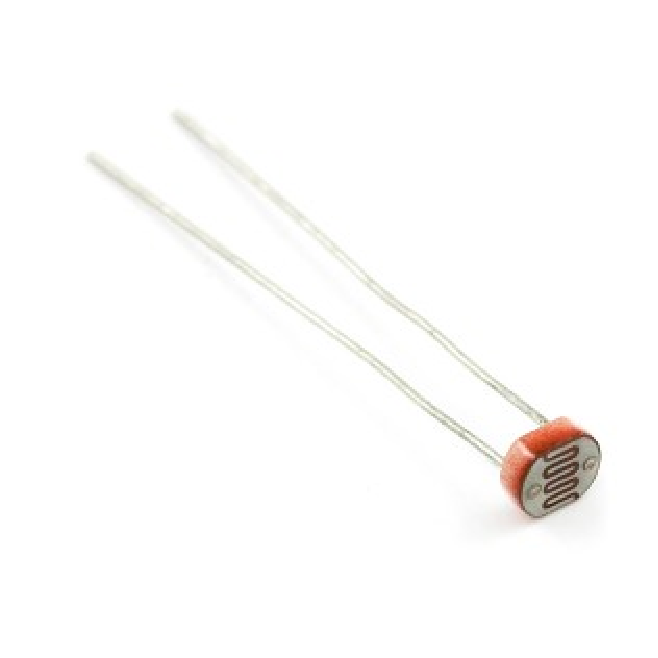
\includegraphics[width=0.3\linewidth]{figures/ldr.eps}
  \caption{LDR}
  \label{fig:blinkingLEDLayout}
\end{figure}

\section{Configuration}
Use X-CTU to configure your XBees.
One of them must be configured as a router (e.g., router AT 22A7 at the time of writing)a and the other as a coordinator API (e.g., coordinator API 21A7 at the time of writing).

For the router, configure the PANID, the destination address (both high and low), enable channel verification (Networking -> JV), set D0 to analog (I/O settings -> D0 -> ADC) and set the sampling rate to 128 ms (I/O settings -> I/O sampling -> IR - I/O sampling rate -> FF).

For the coordinator, you just have to configure the PANID and the destination's address.

\section{Connections}

For prototyping purposes, we will place the sensing and the processing board next to the other as in Fig. \ref{fig:sunset_sensor}, to make it possible to power both of them using the Arduino.
For real deployment, you could use batteries to power the sensor board.

Connect digital outputs 10, 11 and 12 to the LEDs.
Optionally you can also connect a buzzer if you are feeling noisy.

Connect also the LDR in series with a resistor that is twice as much the LDR (20 Kohm).
The input to the XBee is precisely the connection between the LDR and the resistor.

Make sure that the RSSI LEDs of the explorer are on, which means that both of them are in the same network.
Note that we are using the series communication pins to pass information from the XBee to the Arduino.
This wires need to be removed to program the Arduino, as the programming process also uses the serial communication port.



\begin{figure}[htbp]
  \centering
  
\includegraphics[width=0.9\linewidth]{figures/sunset_sensor.eps}
  \caption{Sunset sensor connections}
  \label{fig:sunset_sensor}
\end{figure}


\section{Advanced optional assignment}

If you are willing to do more complicated stuff, try to move the alarm to the sensor board. 
Now the sensor board receives the data, sends it to the processing board for processing, and waits for an instruction from the processing board to ring or light the alarm.

\chapter{Collecting data in a computer}

In this assignment we will use some python libraries to receive the data transmitted by the sunset sensor in a computer instead of the Arduino.
You can use one of the university computers, a laptop or a RaspBerry.

Install the XBee python libraries.

\url{http://pypi.python.org/pypi/XBee/2.0.0}

This code offers an implementation of the XBee serial communication API.

We re-use the processing board of the previous assignment and this time we will connect the XBee that receives the data to the computer using the USB cable.
Remember that in the last assignment it was connected to the Arduino.

\begin{lstlisting} [caption = {Simple code that reads the message that arrive to the XBee.}, language = Python, label = {code:simple-receiver}, numbers = left, escapeinside={@}{@}]

import serial
from xbee import ZigBee

print 'Printing data from remote XBee'

serial_port = serial.Serial('/dev/ttyUSB0', 9600)
zigbee = ZigBee(serial_port)

while True:
    try:
        print zigbee.wait_read_frame()
    except KeyboardInterrupt:
        break

serial_port.close()
\end{lstlisting}

You can see the results of running the program in Fig. \ref{fig:sink_in_server_screenshot_first_test}.

\begin{figure}[htbp]
  \centering
  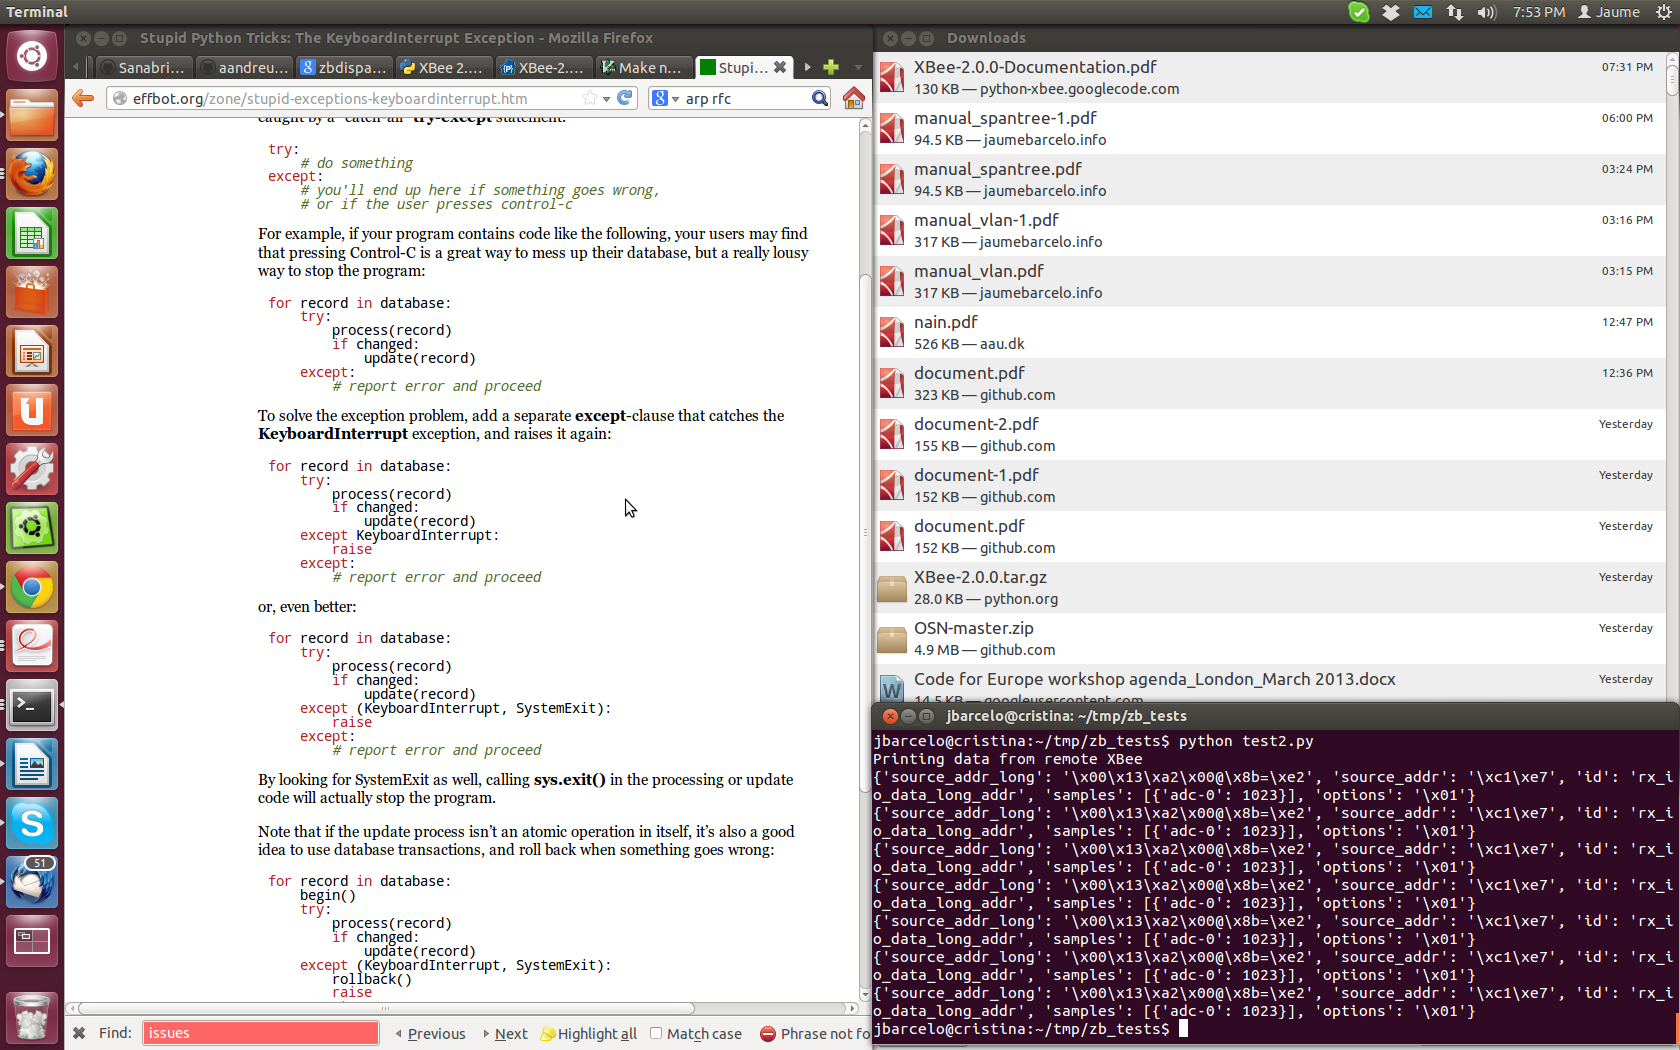
\includegraphics[width=0.7\linewidth]{figures/sink_in_server_screenshot_first_test.eps}
  \caption{A test run of a python program to read the messages that arrive to the XBee.}
  \label{fig:sink_in_server_screenshot_first_test}
\end{figure}



\chapter{Publishing data in cosm}

Create a user in cosm.com .
You will receive an email with a pointer to create an API-Key.
Create this key as you will need it to interact with cosm.

\begin{lstlisting} [caption = {Command to create a feed}, language = sh, label = {code:create-feed}, numbers = left, escapeinside={@}{@}]

curl

\end{lstlisting}

\backmatter
%
\bibliographystyle{plain}
\bibliography{my_bib}
\end{document}
